\section{Bases de datos NoSQL: Documentales (MongoDB)}

Para crear el \textit{cluster} de MongoDB propuesto, también emplearemos las máquinas reales del apartado de Citus. Para ello, necesitaremos 3 nodos; en cada uno se ejecutarán 4 procesos \texttt{mongod} y un proceso \texttt{mongos}. Primero, es necesario instalar y configurar MongoDB.

\subsection*{Instalación y Configuración}

Mediante el siguiente \textit{script Bash}, podemos instalar la versión 6.0 del paquete \texttt{mongo-org} en nuestras máquinas. Un detalle importante de esta versión con respecto a la versión instalada en las máquinas virtuales es que el comando \texttt{mongo} ha sido renombrado a \texttt{mongosh}.

\begin{minted}[frame=single, fontsize=\footnotesize]{bash}
#!/bin/bash

# run from local with: ssh user@host 'bash -s' < <path_to_this_file>

# Importar la clave de mongo al llavero del sistema operativo
wget -qO - https://www.mongodb.org/static/pgp/server-6.0.asc |  gpg --dearmor | \
sudo tee /usr/share/keyrings/mongodb.gpg > /dev/null

# Actualizar el repositorio de apt para incluir mongo-org
echo "deb [ arch=amd64,arm64 signed-by=/usr/share/keyrings/mongodb.gpg ]" \
"https://repo.mongodb.org/apt/ubuntu jammy/mongodb-org/6.0 multiverse" | \
sudo tee /etc/apt/sources.list.d/mongodb-org-6.0.list

# Actualizar el controlador de paquetes del sistema
sudo apt update

# Instalar mongo
sudo apt install -y mongodb-org

# Mostrar versiones instaladas
mongod --version
mongosh --version

# Reiniciar el sistema
sudo reboot
\end{minted}

Para facilitar el manejo de direcciones IP, podemos añadir un alias para las distintas IP de las máquinas en el archivo \texttt{\$HOME/etc/hosts}, lo cual nos permitirá hacer referencia a otros nodos de una forma mucho más cómoda.

\begin{minted}[frame=single, fontsize=\footnotesize]{bash}
#!/bin/bash

HOSTS=(
    "51.210.241.66   ovh1"
    "51.210.241.239  ovh2"
    "51.210.241.207  ovh3"
)

# Añadir pareja {ip: alias} a /etc/hosts si no existen
for ENTRY in "${HOSTS[@]}"; do
  IP=$(echo "${ENTRY}" | awk '{print $1}')
  HOSTNAME=$(echo "${ENTRY}" | awk '{print $2}')
  
  if grep -q "${IP}" /etc/hosts; then
    echo "Entry '${ENTRY}' already exists in /etc/hosts. Skipping."
  else
    echo "Adding '${ENTRY}' to /etc/hosts"
    echo "${ENTRY}" | sudo tee -a /etc/hosts > /dev/null
  fi
done

tail /etc/hosts -n 5
\end{minted}

\subsection*{Lanzamiento de los Procesos de MongoDB}

Para crear nuestro \textit{cluster}, es necesario lanzar un total de 4 procesos \texttt{mongod} y un proceso \texttt{mongos} en cada nodo. Cada proceso tendrá una configuración específica según su rol en el \textit{cluster}. A continuación, se describen los detalles de estos procesos:

\begin{itemize}
    \item \textbf{1 proceso de configuración (\texttt{configsrv})}: Este proceso \texttt{mongod} actúa como el servidor de configuración del \textit{cluster}. Su rol es almacenar los metadatos del \textit{cluster}, como el mapeo de fragmentos y la información de distribución de datos.
    \item \textbf{3 procesos de fragmentos (\texttt{shardsvr})}: Estos procesos \texttt{mongod} se encargan de almacenar los datos reales del \textit{cluster}. Cada uno representa un fragmento diferente del conjunto de datos. Cada fragmento se configurará como un conjunto de réplicas para mejorar la redundancia y disponibilidad.
    \item \textbf{1 proceso de enrutamiento (\texttt{mongos})}: Este proceso actúa como el enrutador del \textit{cluster}. Es el encargado de recibir las solicitudes de los clientes y dirigirlas a los fragmentos correspondientes. Debe configurarse para conectarse a los servidores de configuración (\texttt{configsvr}) y proporciona un punto de entrada único para las operaciones del cliente, ocultando la complejidad interna del \textit{cluster}.
\end{itemize}

Para lanzar estos procesos, podemos hacerlo desde la terminal especificando las distintas opciones como argumentos, o podemos crear archivos de configuración específicos para cada proceso. Optamos por la segunda vía, definiendo los siguientes archivos de configuración: \\

\noindent \textbf{Archivo de Configuración para el Config Server}

\begin{minted}[frame=single, fontsize=\footnotesize]{yaml}
sharding:
  clusterRole: configsvr
  
replication:
  replSetName: rsConfServer

storage:
  dbPath: /home/ubuntu/dbMongo/rsConfServer

systemLog:
  destination: file
  logAppend: true
  path: /home/ubuntu/dbMongo/rsConfServer/mongod.log

net:
  port: 27010
  bindIp: 0.0.0.0

processManagement:
  timeZoneInfo: /usr/share/zoneinfo
  fork: true

security:
  keyFile: /home/ubuntu/mongo_keyfile
  authorization: enabled
\end{minted}
\newpage 

\noindent \textbf{Archivo de Configuración para los Shards:} para cada uno de los 3 \textit{shards}, el archivo de configuración sería el siguiente. Solo cambia el nombre del conjunto de réplicas (\texttt{replSetName}), las rutas a los directorios donde se guardarán los datos, los \textit{logs} y el puerto (\texttt{net.port}) para cada \textit{shard}.

\begin{minted}[frame=single, fontsize=\footnotesize]{yaml}
sharding:
  clusterRole: shardsvr
  
replication:
  replSetName: rsShard{1|2|3}

storage:
  dbPath: /home/ubuntu/dbMongo/rsShard{1|2|3}

systemLog:
  destination: file
  logAppend: true
  path: /home/ubuntu/dbMongo/rsShard{1|2|3}/mongod.log

net:
  port: {27011 | 27012 | 27013}
  bindIp: 0.0.0.0

processManagement:
  timeZoneInfo: /usr/share/zoneinfo
  fork: true

security:
  keyFile: /home/ubuntu/mongo_keyfile
  authorization: enabled
\end{minted}

\noindent \textbf{Archivo de Configuración para el Proceso Mongos} 

\begin{minted}[frame=single, fontsize=\footnotesize]{yaml}
sharding:
  configDB: rsConfServer/ovh1:27010,ovh2:27010,ovh3:27010

processManagement:
  timeZoneInfo: /usr/share/zoneinfo
  fork: true

security:
  keyFile: /home/ubuntu/mongo_keyfile

systemLog:
  destination: file
  logAppend: true
  path: /home/ubuntu/dbMongo/mongos/mongod.log

net:
  port: 27017
  bindIp: 0.0.0.0
\end{minted}

\noindent A continuación, se explican las diferentes opciones de configuración:

\begin{enumerate}
    \item \textbf{sharding.clusterRole}: 
    \begin{itemize}
        \item Define el rol de cada nodo dentro del \textit{cluster} de \textit{sharding}. Puede ser \texttt{configsvr} (servidor de configuración) o \texttt{shardsvr} (shard). El proceso \texttt{mongos} no tiene esta opción.
    \end{itemize}
    \item \textbf{replication.replSetName}: 
    \begin{itemize}
        \item Especifica el nombre del conjunto de réplicas para los nodos de replicación. Los nodos de los \textit{shards} y el \texttt{config server} estarán en conjuntos de réplicas, lo que garantiza la disponibilidad y la redundancia de los datos.
    \end{itemize}
    \item \textbf{storage.dbPath}: 
    \begin{itemize}
        \item Define la ruta en el sistema de archivos donde MongoDB almacenará los datos de la base de datos. Cada componente tiene su propia ruta específica (por ejemplo, \texttt{rsConfServer} para el \texttt{config server} y \texttt{rsShard1}, \texttt{rsShard2}, \texttt{rsShard3} para los shards).
    \end{itemize}
    \item \textbf{systemLog.destination y systemLog.path}: 
    \begin{itemize}
        \item Configuran donde se almacenarán los \textit{logs} del sistema de MongoDB. En este caso, se almacenan en archivos de \textit{log} dentro de un directorio específico.
        \item \texttt{logAppend} asegura que los \textit{logs} se agreguen al archivo existente, evitando sobrescribir los \textit{logs} anteriores.
    \end{itemize}
    \item \textbf{net.port y net.bindIp}: 
    \begin{itemize}
        \item Configuran el puerto y las interfaces de red en las que MongoDB escuchará las conexiones. \texttt{bindIp: 0.0.0.0} permite que el servicio escuche en todas las interfaces de red, abriendo el servidor al tráfico externo.
    \end{itemize}
    \item \textbf{processManagement.fork}: 
    \begin{itemize}
        \item \texttt{fork} indica que el proceso de MongoDB se ejecutará en segundo plano como un \textit{daemon} después de iniciarse correctamente y nos devolverá la terminal. Para habilitar esta opción es necesario configurar el guardado de \textit{logs}.
    \end{itemize}
    \item \textbf{security.keyFile y security.authorization}: 
    \begin{itemize}
        \item \texttt{keyFile}: Define el archivo de clave compartida que MongoDB usará para autenticar y asegurar la comunicación entre los diferentes nodos del \textit{cluster}.
        \item \texttt{authorization}: Activa la autenticación de usuarios, lo que significa que los clientes también deben autenticarse para acceder a las bases de datos de MongoDB.
    \end{itemize}
\end{enumerate}

Ahora debemos distribuir los archivos de configuración y el archivo \texttt{keyFile} usado para autenticar la comunicación entre los nodos a las tres máquinas. Para ello, utilizamos el siguiente \textit{script bash}:

\begin{minted}[frame=single, fontsize=\footnotesize]{bash}
#!/bin/bash

# Rutas de archivos y carpetas
MONGO_KEYFILE_NAME="mongo_keyfile"
MONGO_KEYFILE="./4.mongo/setup/${MONGO_KEYFILE_NAME}"
MONGO_CONFIGS="./4.mongo/setup/configs/*"
MONGO_CONFIGS_PATH="/home/ubuntu/mongo/config/"
MONGO_DB_PATH="/home/ubuntu/dbMongo/"

# Hosts
REMOTE_HOSTS=("ovh1" "ovh2" "ovh3")

for REMOTE_HOST in "${REMOTE_HOSTS[@]}"; do

  ssh "$REMOTE_HOST" "sudo rm -r $MONGO_DB_PATH"

  # Crear los directorios necesarios en cada máquina
  ssh "$REMOTE_HOST" "mkdir -p ${MONGO_CONFIGS_PATH}"
  ssh "$REMOTE_HOST" "mkdir -p ${MONGO_DB_PATH}/rsConfServer"
  ssh "$REMOTE_HOST" "mkdir -p ${MONGO_DB_PATH}/rsShard1"
  ssh "$REMOTE_HOST" "mkdir -p ${MONGO_DB_PATH}/rsShard2"
  ssh "$REMOTE_HOST" "mkdir -p ${MONGO_DB_PATH}/rsShard3"
  ssh "$REMOTE_HOST" "mkdir -p ${MONGO_DB_PATH}/mongos"

  # Copiar el archivo keyFile
  scp "$MONGO_KEYFILE" "${REMOTE_HOST}:~/"

  # Copiar los archivos de configuración
  scp $MONGO_CONFIGS "${REMOTE_HOST}:${MONGO_CONFIGS_PATH}"

  # Dar permisos de lectura y escritura para el archivo keyFile
  ssh "$REMOTE_HOST" "sudo chmod 600 ~/$MONGO_KEYFILE_NAME"

done
\end{minted}

\noindent Este script realiza los siguientes pasos:
\begin{enumerate}
    \item Elimina el directorio de base de datos existente en cada máquina, si existe.
    \item Crea los directorios necesarios en cada máquina para almacenar las configuraciones y los datos de MongoDB.
    \item Copia el archivo \texttt{keyFile} a cada máquina para garantizar la autenticación segura entre los nodos.
    \item Copia los archivos de configuración de MongoDB a cada máquina.
    \item Asigna los permisos adecuados al archivo \texttt{keyFile}.
\end{enumerate}

\subsubsection*{Levantamiento de los Procesos en el Cluster}

Ahora que los archivos de configuración y el archivo \texttt{keyFile} están distribuidos, podemos proceder a levantar los procesos necesarios para el \textit{cluster} de MongoDB. El primer paso es iniciar el \textit{replicaset} del servidor de configuración.

\subsubsection*{Iniciar el ReplicaSet de Configuración}

En cada máquina, ejecutamos el siguiente comando para iniciar el proceso \texttt{mongod} con el archivo de configuración para el servidor de configuración:

\begin{minted}[frame=single, fontsize=\footnotesize]{bash}
mongod --config mongo/config/configsvr.conf
\end{minted}

\noindent En solo una máquina, nos conectamos a la \textit{shell} de MongoDB usando \texttt{mongosh}:

\begin{minted}[frame=single, fontsize=\footnotesize]{bash}
mongosh --port 27010
\end{minted}

\noindent Dentro de la shell de MongoDB, iniciamos el \textit{replicaset} del servidor de configuración:

\begin{minted}[frame=single, fontsize=\footnotesize]{javascript}
rs.initiate(
  {
    _id: "rsConfServer",
    configsvr: true,
    members: [
      { _id : 0, host : "ovh1:27010" },
      { _id : 1, host : "ovh2:27010" },
      { _id : 2, host : "ovh3:27010" }
    ]
  }
)
\end{minted}

\noindent Una vez iniciado el servidor de configuración, podemos proceder a lanzar los procesos de los \textit{shards}.

\subsubsection*{Iniciar los Procesos de los Shards}

En cada máquina, ejecutamos los siguientes comandos para iniciar los procesos de los tres \textit{shards}:

\begin{minted}[frame=single, fontsize=\footnotesize]{bash}
mongod --config mongo/config/shard1.conf
mongod --config mongo/config/shard2.conf
mongod --config mongo/config/shard3.conf
\end{minted}

\noindent Luego, en solo una máquina, nos conectamos a cada uno de los \textit{replicates} para inicializarlos.

\begin{minted}[frame=single, fontsize=\footnotesize]{bash}
mongosh --port 27011
\end{minted}

\noindent Dentro de la \textit{shell} de MongoDB, inicializamos el \textit{replicaset} para el primer \textit{shard}:

\begin{minted}[frame=single, fontsize=\footnotesize]{javascript}
rs.initiate(
  {
    _id : "rsShard1",
    members: [
      { _id : 0, host : "ovh1:27011" },
      { _id : 1, host : "ovh2:27011" },
      { _id : 2, host : "ovh3:27011" }
    ]
  }
)
\end{minted}

\noindent Realizamos el mismo proceso para los otros dos \textit{shards}:

\begin{minted}[frame=single, fontsize=\footnotesize]{bash}
mongosh --port 27012
rs.initiate(
  {
    _id : "rsShard2",
    members: [
      { _id : 0, host : "ovh1:27012" },
      { _id : 1, host : "ovh2:27012" },
      { _id : 2, host : "ovh3:27012" }
    ]
  }
)
\end{minted}

\begin{minted}[frame=single, fontsize=\footnotesize]{bash}
mongosh --port 27013
rs.initiate(
  {
    _id : "rsShard3",
    members: [
      { _id : 0, host : "ovh1:27013" },
      { _id : 1, host : "ovh2:27013" },
      { _id : 2, host : "ovh3:27013" }
    ]
  }
)
\end{minted}

\subsubsection*{Lanzar el Proceso Mongos}

Finalmente, lanzamos el proceso \texttt{mongos} en una máquina con la siguiente configuración:

\begin{minted}[frame=single, fontsize=\footnotesize]{bash}
mongos --config mongo/config/mongos.conf
\end{minted}

\noindent Nos conectamos al enrutador y configuramos los diferentes \textit{shards} del \textit{cluster}:

\begin{minted}[frame=single, fontsize=\footnotesize]{bash}
mongosh --port 27017
sh.addShard( "rsShard1/ovh1:27011,ovh2:27011,ovh3:27011")
sh.addShard( "rsShard2/ovh1:27012,ovh2:27012,ovh3:27012")
sh.addShard( "rsShard3/ovh1:27013,ovh2:27013,ovh3:27013")
\end{minted}

\subsubsection*{Habilitar Autenticación y Crear un Usuario}

Un detalle importante es que la autenticación tuvo que deshabilitarse para permitir la conexión con \texttt{mongosh} durante la configuración del \textit{cluster}. Una vez que el \textit{cluster} esté creado, nos conectamos y creamos un usuario privilegiado con los siguientes comandos:

\begin{minted}[frame=single, fontsize=\footnotesize]{javascript}
db.createUser({
  user: "admin",
  pwd: "***",
  roles: [
    { role: "userAdminAnyDatabase", db: "admin" },
    { role: "clusterAdmin", db: "admin" },
    { role: "readWriteAnyDatabase", db: "admin" }
  ]
});
\end{minted}

Finalmente, debemos parar todos los procesos \texttt{mongod} y \texttt{mongos} en todas las máquinas utilizando el siguiente comando:

\begin{minted}[frame=single, fontsize=\footnotesize]{bash}
pkill -9 mongo
\end{minted}

En la figura \ref{fig:matar_mongo} mostramos la verificación de que no existen procesos \texttt{mongod} o \texttt{mongos} en ejecución con el siguiente comando:

\begin{minted}[frame=single, fontsize=\footnotesize]{bash}
pgrep mongo
\end{minted}

\begin{figure}[H]
\centering
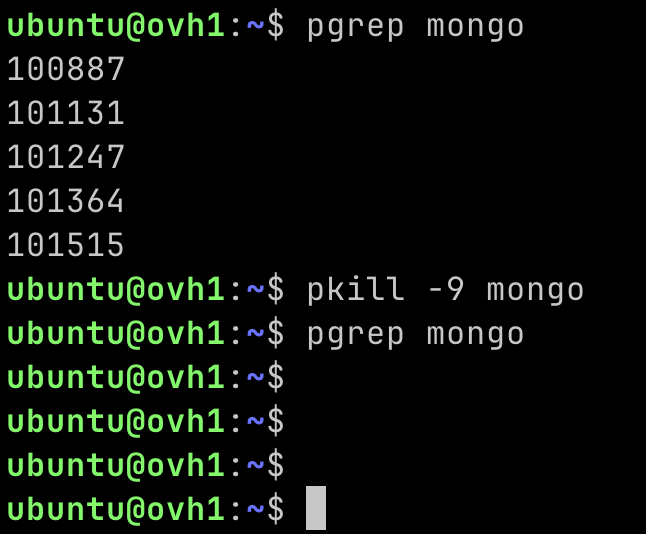
\includegraphics[width=0.3\textwidth]{fotos/mongo/matar_mongo.png}
\caption{Verificación de procesos \textit{mongod} en ejecución}
\label{fig:matar_mongo}
\end{figure}

Rehabilitamos la autenticación, y luego volvemos a lanzar los procesos \texttt{mongod} y \texttt{mongos}. Esta vez no es necesario inicializar los \textit{replicaSets} o agregar los \textit{shards}, ya que el \textit{cluster} mantiene los datos de configuración. Esto lo vemos en la figura \ref{fig:lanzar_mongo}.

\begin{figure}[H]
\centering
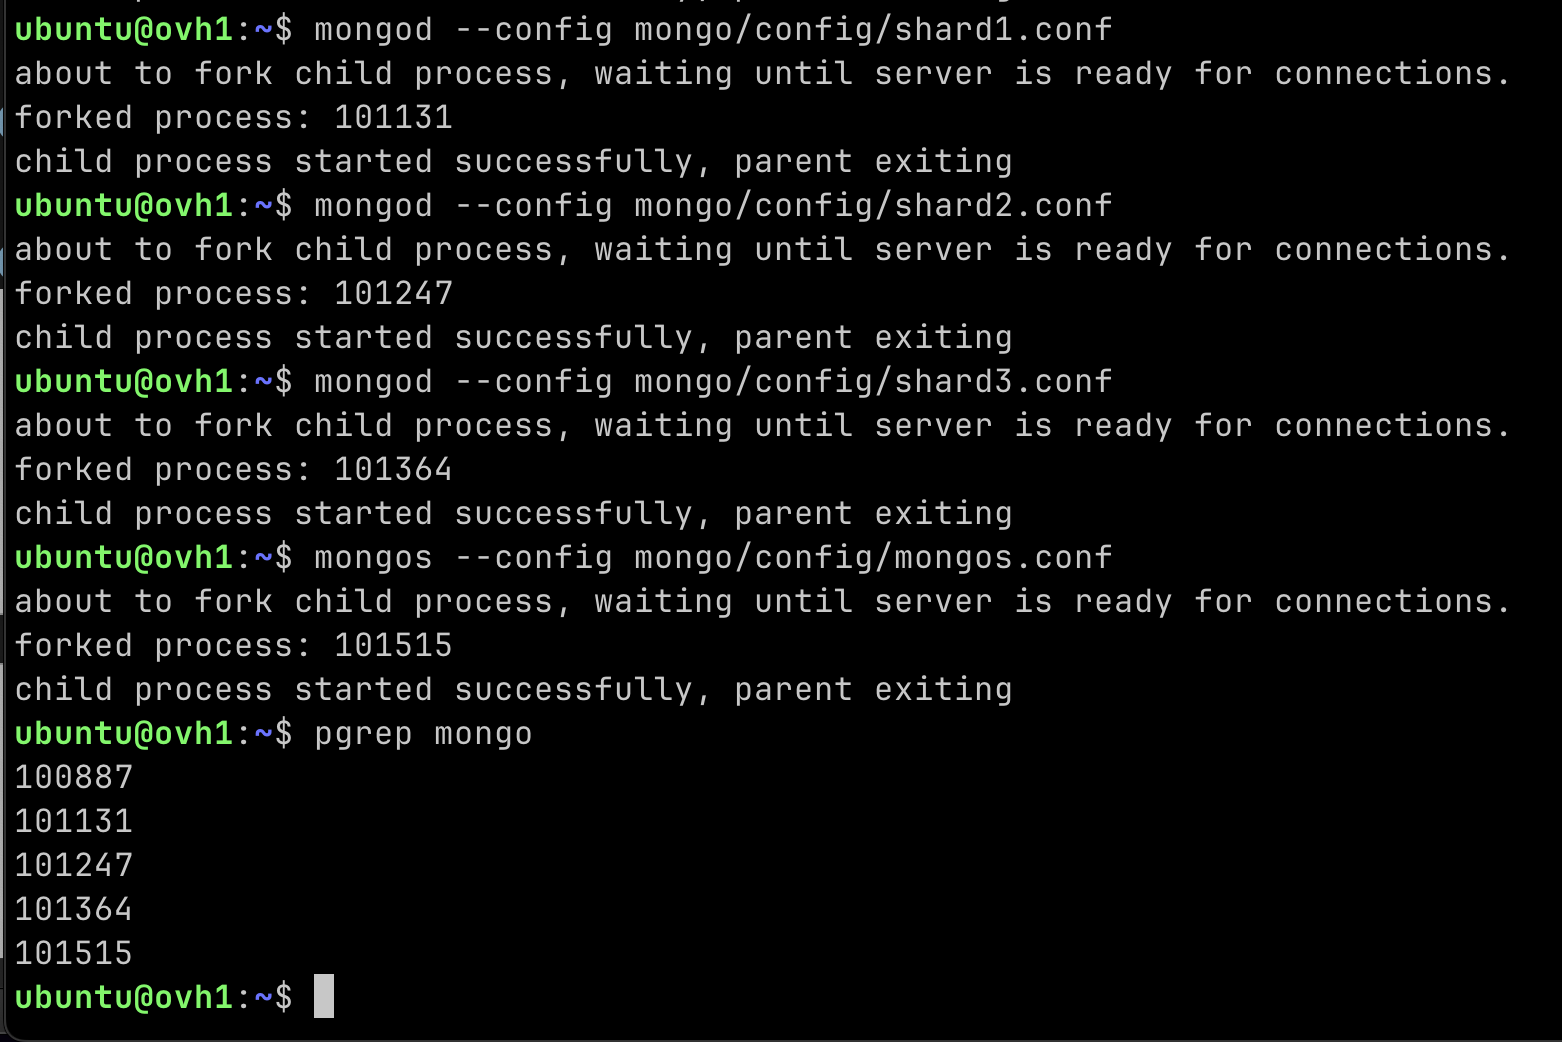
\includegraphics[width=0.6\textwidth]{fotos/mongo/lanzar_mongod.png}
\caption{Lanzamiento de los procesos \textit{mongod} y \textit{mongos}.}
\label{fig:lanzar_mongo}
\end{figure}


\subsection{Extracción de datos para consultas Q1 y Q3}

En la práctica se nos pide diseñar una colección que permita resolver de forma eficiente las consultas Q1 y Q3, consultas centradas en partidos de torneos específicos. Diseñamos, pues, esta colección partiendo de la tabla de partidos, y agregando a cada partido todas las demás tablas, excepto la tabla de \textit{ranking}. \\

En nuestra base de datos relacional, ejecutamos la siguiente instrucción SQL para generar un archivo que contenga los diferentes documentos JSON que importaremos a MongoDB:

\begin{minted}[frame=single, fontsize=\footnotesize]{sql}
COPY (
    SELECT 
        jsonb_build_object(
            'torneo', jsonb_build_object(
                'id', t.id,
                'nombre', t.nombre,
                'fecha', et.fecha,
                'pais', CASE 
                            WHEN tp.codigo_iso2 IS NOT NULL THEN jsonb_build_object(
                                'codigo_iso2', tp.codigo_iso2,
                                'codigo_iso3', tp.codigo_iso3,
                                'codigo_ioc', tp.codigo_ioc,
                                'nombre', tp.nombre
                            )
                            ELSE NULL 
                        END,
                'superficie', et.superficie,
                'tamano', et.tamano,
                'nivel', et.nivel
            ),
            'num_sets', p.num_sets,
            'ronda', p.ronda,
            'desenlace', p.desenlace,
            'ganador', CASE 
                           WHEN jg.id IS NOT NULL THEN jsonb_build_object(
                               'id', jg.id,
                               'nombre', jg.nombre,
                               'apellido', jg.apellido,
                               'diestro', jg.diestro,
                               'fecha_nacimiento', jg.fecha_nacimiento,
                               'altura', jg.altura,
                               'pais', CASE 
                                           WHEN pg.codigo_iso2 IS NOT NULL THEN jsonb_build_object(
                                               'codigo_iso2', pg.codigo_iso2,
                                               'codigo_iso3', pg.codigo_iso3,
                                               'codigo_ioc', pg.codigo_ioc,
                                               'nombre', pg.nombre
                                           )
                                           ELSE NULL 
                                       END,
                               'stats', jsonb_build_object(
                                   'aces', p.num_aces_ganador,
                                   'dobles_faltas', p.num_dob_faltas_ganador,
                                   'puntos_servidos', p.num_ptos_servidos_ganador,
                                   'primeros_servicios', p.num_primeros_servicios_ganador,
                                   'primeros_servicios_ganados', p.num_primeros_servicios_ganados_ganador,
                                   'segundos_servicios_ganados', p.num_segundos_servicios_ganados_ganador,
                                   'juegos_servidos', p.num_juegos_servidos_ganador,
                                   'breaks_salvados', p.num_break_salvados_ganador,
                                   'breaks_afrontados', p.num_break_afrontados_ganador
                               )
                           )
                           ELSE NULL 
                       END,
            'perdedor', CASE 
                            WHEN jp.id IS NOT NULL THEN jsonb_build_object(
                                'id', jp.id,
                                'nombre', jp.nombre,
                                'apellido', jp.apellido,
                                'diestro', jp.diestro,
                                'fecha_nacimiento', jp.fecha_nacimiento,
                                'altura', jp.altura,
                                'pais', CASE 
                                            WHEN pp.codigo_iso2 IS NOT NULL THEN jsonb_build_object(
                                                'codigo_iso2', pp.codigo_iso2,
                                                'codigo_iso3', pp.codigo_iso3,
                                                'codigo_ioc', pp.codigo_ioc,
                                                'nombre', pp.nombre
                                            )
                                            ELSE NULL 
                                        END,
                                'stats', jsonb_build_object(
                                    'aces', p.num_aces_perdedor,
                                    'dobles_faltas', p.num_dob_faltas_perdedor,
                                    'puntos_servidos', p.num_ptos_servidos_perdedor,
                                    'primeros_servicios', p.num_primeros_servicios_perdedor,
                                    'primeros_servicios_ganados', p.num_primeros_servicios_ganados_perdedor,
                                    'segundos_servicios_ganados', p.num_segundos_servicios_ganados_perdedor,
                                    'juegos_servidos', p.num_juegos_servidos_perdedor,
                                    'breaks_salvados', p.num_break_salvados_perdedor,
                                    'breaks_afrontados', p.num_break_afrontados_perdedor
                                )
                            )
                            ELSE NULL 
                        END,
            'sets', (
                SELECT jsonb_agg(
                    jsonb_build_object(
                        'num_set', sp.num_set,
                        'juegos_ganador', sp.juegos_ganador,
                        'juegos_perdedor', sp.juegos_perdedor,
                        'puntos_tiebreak_perdedor', sp.puntos_tiebreak_perdedor
                    )
                )
                FROM sets_partido sp
                WHERE sp.torneo = p.torneo AND sp.fecha = p.fecha AND sp.num_partido = p.num_partido
            )
        )
    FROM 
        partido p
        JOIN edicion_torneo et ON p.torneo = et.torneo AND p.fecha = et.fecha
        JOIN torneo t ON et.torneo = t.id
        LEFT JOIN pais tp ON t.pais = tp.codigo_iso2
        LEFT JOIN jugador jg ON p.ganador = jg.id
        LEFT JOIN pais pg ON jg.pais = pg.codigo_iso2
        LEFT JOIN jugador jp ON p.perdedor = jp.id
        LEFT JOIN pais pp ON jp.pais = pp.codigo_iso2
) TO '/tmp/tenis.json';
\end{minted}

\noindent Al ejecutarla, nos genera el archivo \texttt{tenis.json}, que contiene documentos JSON con el siguiente formato:

\begin{minted}[frame=single, fontsize=\footnotesize]{json}
{
  "sets": [
    {
      "num_set": 1,
      "juegos_ganador": 6,
      "juegos_perdedor": 4,
      "puntos_tiebreak_perdedor": null
    },
    {
      "num_set": 2,
      "juegos_ganador": 5,
      "juegos_perdedor": 7,
      "puntos_tiebreak_perdedor": null
    },
    {
      "num_set": 3,
      "juegos_ganador": 6,
      "juegos_perdedor": 4,
      "puntos_tiebreak_perdedor": null
    }
  ],
  "ronda": "R32",
  "torneo": {
    "id": 112,
    "pais": {
      "nombre": "United Kingdom",
      "codigo_ioc": "GBR",
      "codigo_iso2": "GB",
      "codigo_iso3": "GBR"
    },
    "fecha": "2019-07-07",
    "nivel": "A",
    "nombre": "Newport",
    "tamano": 32,
    "superficie": "Hierba"
  },
  "ganador": {
    "id": 105815,
    "pais": {
      "nombre": "United States of America",
      "codigo_ioc": "USA",
      "codigo_iso2": "US",
      "codigo_iso3": "USA"
    },
    "stats": {
      "aces": 8,
      "dobles_faltas": 4,
      "breaks_salvados": 4,
      "juegos_servidos": 16,
      "puntos_servidos": 113,
      "breaks_afrontados": 6,
      "primeros_servicios": 57,
      "primeros_servicios_ganados": 46,
      "segundos_servicios_ganados": 25
    },
    "altura": 188,
    "nombre": "Tennys",
    "diestro": true,
    "apellido": "Sandgren",
    "fecha_nacimiento": "1991-07-07"
  },
  "num_sets": 3,
  "perdedor": {
    "id": 104797,
    "pais": {
      "nombre": "Uzbekistan",
      "codigo_ioc": "UZB",
      "codigo_iso2": "UZ",
      "codigo_iso3": "UZB"
    },
    "stats": {
      "aces": 1,
      "dobles_faltas": 4,
      "breaks_salvados": 5,
      "juegos_servidos": 16,
      "puntos_servidos": 101,
      "breaks_afrontados": 8,
      "primeros_servicios": 60,
      "primeros_servicios_ganados": 43,
      "segundos_servicios_ganados": 20
    },
    "altura": 188,
    "nombre": "Denis",
    "diestro": true,
    "apellido": "Istomin",
    "fecha_nacimiento": "1986-09-09"
  },
  "desenlace": "N"
}
\end{minted}

\subsection{Indexación, sharding y carga de datos}

A la hora de distribuir los datos, debemos también indexar el atributo que vayamos a utilizar como clave de partición. Elegimos indexar y particionar por el atributo \texttt{torneo.nombre} mediante \textit{hash}, ya que es empleado en casi todas las consultas y presenta una alta cardinalidad. Deberemos comprobar, después de importar los documentos, cuántos \textit{chunks} guarda cada \textit{shard} para verificar que existe un reparto equitativo. Ajustamos el valor del tamaño de \textit{chunks}, por defecto 128 \textit{megabytes} en MongoDB 6.0, a un tamaño de 8 megas, para forzar la distribución de los datos entre todos los \textit{shards}:

\newpage

\begin{minted}[frame=single, fontsize=\footnotesize]{js}
use tenis

db.createCollection('partidos')

db.settings.updateOne(
   { _id: "chunksize" },
   { $set: { _id: "chunksize", value: 8 } },
   { upsert: true }
)

db.partidos.createIndex({"torneo.nombre": "hashed"})
sh.shardCollection("tenis.partidos", {"torneo.nombre":"hashed"})
\end{minted}

\noindent Generamos y cargamos los datos desde ovh1:

\begin{minted}[frame=single, fontsize=\footnotesize]{bash}
psql service=citus -f 4.mongo/sql_to_json.sql
mongoimport --host ovh1 --port 27017 --db tenis2 --collection partidos --file /tmp/tenis.json --authenticationDatabase admin -u admin -p ***
\end{minted}

\noindent Debemos verificar que nuestro \textit{cluster} ha reparticionado los datos de forma equitativa entre todos los nodos. Esto lo vemos en la figura \ref{fig:chunks} y lo hacemos con el siguiente comando:

\begin{minted}[frame=single, fontsize=\footnotesize]{js}
sh.status()
\end{minted}

\begin{figure}[H]
\centering
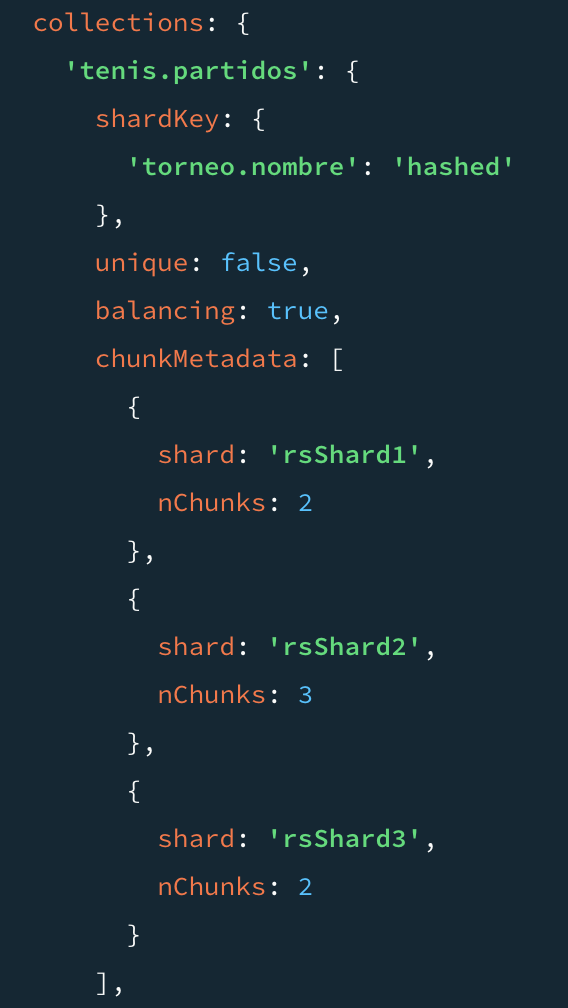
\includegraphics[width=0.3\textwidth]{fotos/mongo/chunks.png}
\caption{Verificación del reparto equitativo de los datos en los nodos del cluster en MongoDB.}
\label{fig:chunks}
\end{figure}




\newpage

\subsection{Consultas MongoDB}

\subsubsection{Muestra todos los ganadores del torneo ``Wimbledon'' (Nombre apellidos y año). Ordena el resultado por año.}

Esta consulta (cuyo resultado vemos en la figura \ref{fig:q1_mongo}) está compuesta por tres etapas en un \texttt{pipeline} de agregación:

\begin{enumerate}
    \item \textbf{\$match:} Filtramos los documentos para incluir solo aquellos del torneo ``Wimbledon'' y de la ronda final (`F').
    \item \textbf{\$project:} Seleccionamos los campos que se mostrarán en el resultado. En este caso:
    \begin{itemize}
        \item Excluye el campo \_id.
        \item Muestra el nombre y apellido del ganador.
        \item Extrae y muestra el año de la fecha del torneo.
    \end{itemize}
    
    \item \textbf{\$sort:} Ordenamos los documentos por el año de forma ascendente.
\end{enumerate}

\begin{minted}[frame=single, fontsize=\footnotesize]{js}
db.partidos.aggregate([
  {
    $match: {
      "torneo.nombre": "Wimbledon",
      ronda: "F",
    },
  },
  {
    $project: {
      _id: 0,
      nombre: "$ganador.nombre",
      apellido: "$ganador.apellido",
      año: {
        $year: {
          $toDate: "$torneo.fecha",
        },
      },
    },
  },
  {
    $sort: {
      año: 1,
    },
  },
]);
\end{minted}

\begin{figure}[H]
\centering
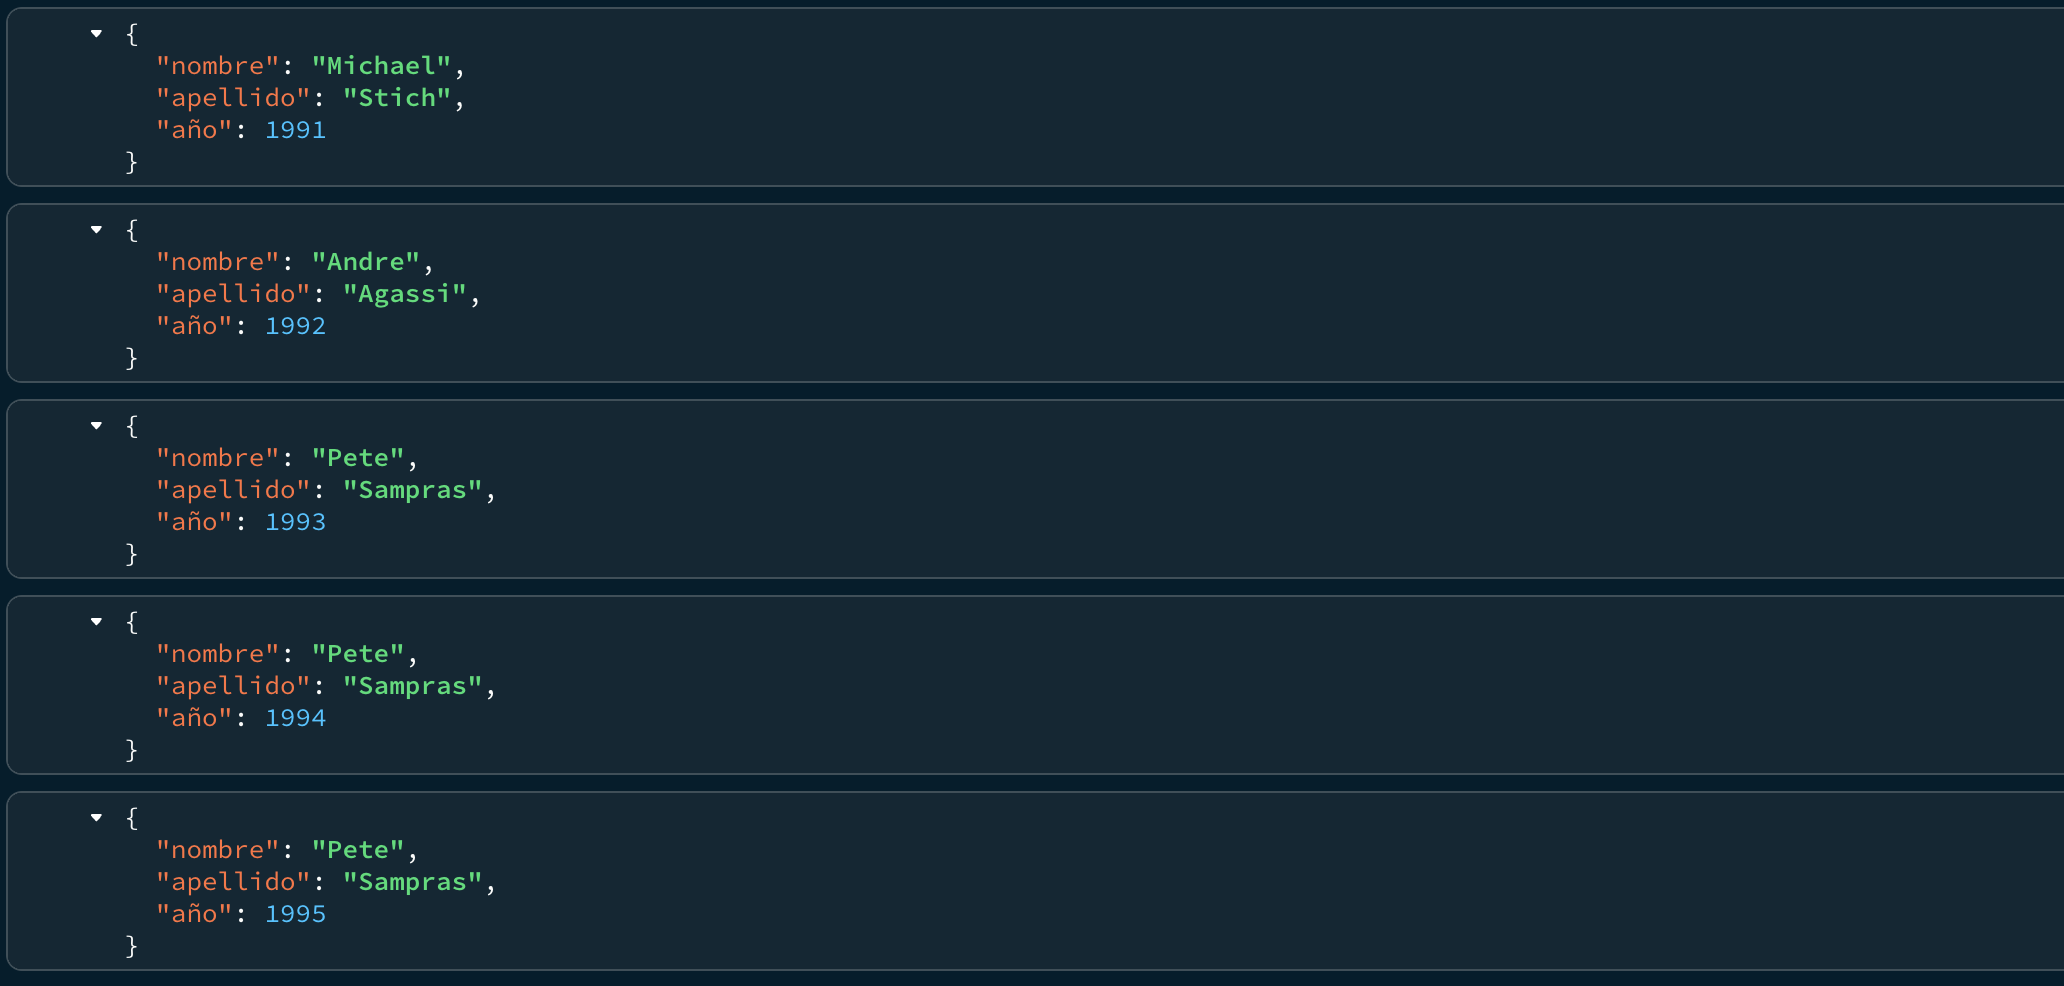
\includegraphics[width=0.6\textwidth]{fotos/mongo/q1.png}
\caption{Bases de datos NoSQL. MongoDB, consulta 1. Al no caber en la propia pantalla, mostramos parte del resultado.}
\label{fig:q1_mongo}
\end{figure}


\subsubsection{Muestra los años en los que Roger Federer ganó algún torneo de nivel Gran Slam (G) o Master 1000 (M). Para cada año, muestra el número de torneos y lista sus nombres (ordenados por la fecha de celebración). Ordena el resultado por el año}

Esta consulta (cuyo resultado mostramos en la figura \ref{fig:q2_mongo}) consta de seis etapas en el \texttt{pipeline} de agregación:

\begin{enumerate}
    \item \textbf{\$match:} Filtramos los documentos para incluir solo aquellos en los que el apellido del ganador es "Federer", el nivel del torneo está en los valores "G" o "M", y la ronda es la final ("F").
    \item \textbf{\$addFields:} Agregamos un nuevo campo \texttt{año}, que contiene el año extraído de la fecha del torneo.
    \item \textbf{\$group:} Agrupamos los documentos por el campo \texttt{año}, contando el total de torneos por año (\texttt{total}), y construimos un \textit{array} de torneos (\texttt{torneos}) con el nombre y la fecha de cada torneo.
    \item \textbf{\$addFields:} Dentro de la etapa de agregar campos, ordenamos el \textit{array} de torneos por la fecha de celebración del torneo de manera ascendente.
    \item \textbf{\$project:} Proyectamos los campos del resultado final. Excluimos el campo \_id, pero mostramos el año y el total de torneos por año. Además, convertimos el \textit{array} de torneos en una cadena de texto separada por comas, listando los nombres de los torneos en orden.
    \item \textbf{\$sort:} Ordenamos los resultados por el campo \texttt{año} de manera ascendente.
\end{enumerate}

\begin{minted}[frame=single, fontsize=\footnotesize]{js}
db.partidos.aggregate([
  {
    $match: {
      "ganador.apellido": "Federer",
      "torneo.nivel": { $in: ["G", "M"] },
      ronda: "F",
    },
  },
  {
    $addFields: {
      año: {
        $year: { $toDate: "$torneo.fecha" },
      },
    },
  },
  {
    $group: {
      _id: "$año",
      total: { $sum: 1 },
      torneos: {
        $push: {
          nombre: "$torneo.nombre",
          fecha: { $toDate: "$torneo.fecha" },
        },
      },
    },
  },
  {
    $addFields: {
      torneos: {
        $sortArray: {
          input: "$torneos",
          sortBy: { fecha: 1 },
        },
      },
    },
  },
  {
    $project: {
      _id: 0,
      año: "$_id",
      total: "$total",

      torneos: {
        $reduce: {
          input: "$torneos.nombre",
          initialValue: "",
          in: {
            $cond: {
              if: { $eq: ["$$value", ""] },
              then: "$$this",
              else: {
                $concat: ["$$value", ", ", "$$this"],
              },
            },
          },
        },
      },
    },
  },
  {
    $sort: { año: 1 },
  },
]);
\end{minted}

\begin{figure}[H]
\centering
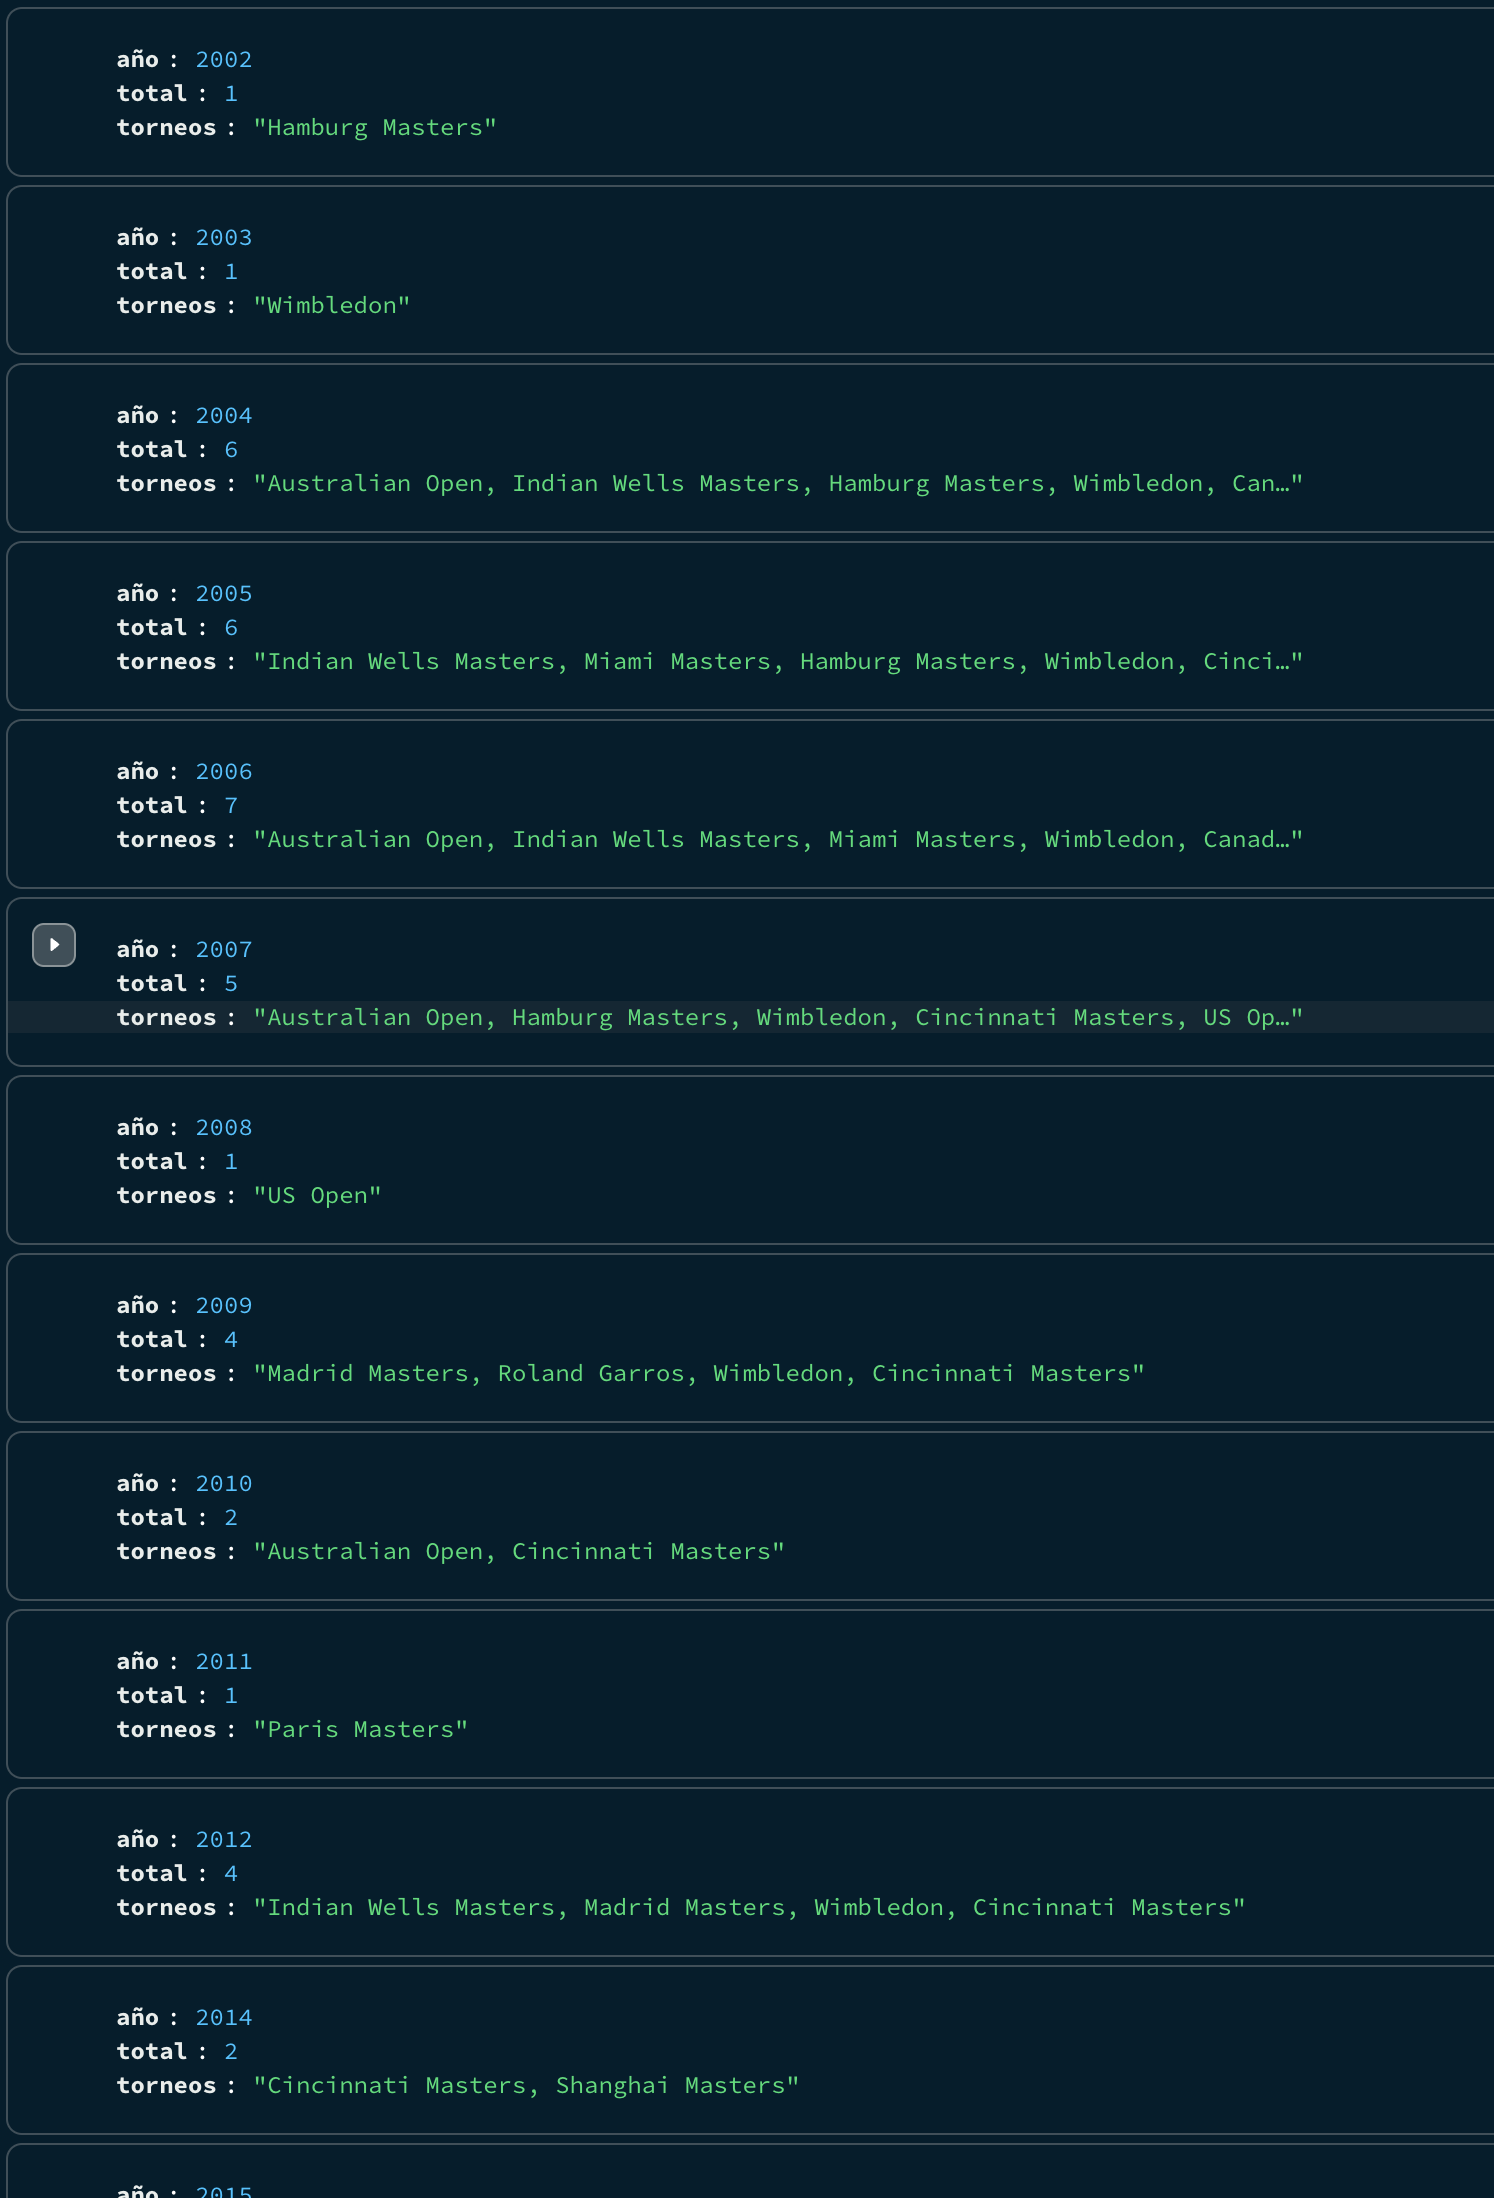
\includegraphics[width=0.45\textwidth]{fotos/mongo/q2.png}
\caption{Bases de datos NoSQL. MongoDB, consulta 2.}
\label{fig:q2_mongo}
\end{figure}


\subsubsection{Muestra los partidos de semifinales (ronda='SF') y final (ronda = 'F') del torneo de "Roland Garros" del 2018. Para cada partido muestra la ronda, el tipo de desenlace, el nombre y apellidos del ganador y el nombre y apellidos del perdedor y el resultado con el número de juegos del ganador y del perdedor en cada set, y opcionalmente en paréntesis el número de juegos del perdedor en el tie break}

Esta consulta (cuyo resultado vemos en la figura \ref{fig:q3_mongo}) consta de tres etapas en el \texttt{pipeline} de agregación:

\begin{enumerate}
    \item \textbf{\$match:} Filtramos los documentos para obtener los partidos del torneo \texttt{"Roland Garros"} que se jugaron en el año 2018. Además, seleccionamos solo los partidos que se juegan en las rondas \texttt{SF} (semifinal) o \texttt{F} (final).
    \item \textbf{\$addFields:} Agregamos un campo nuevo llamado \texttt{resultado} que concatena los resultados de los sets del partido en el siguiente formato: \texttt{juegos\_ganador-juegos\_perdedor}. Si el set contiene puntos de \textit{tiebreak} para el perdedor, los incluimos entre paréntesis después del marcador, y si no hay \textit{tiebreak}, se omite. Este campo contiene la cadena de resultados de todos los sets jugados en el partido.
    \item \textbf{\$project:} Proyectamos los campos seleccionados en el resultado final. Excluyimos el campo \_id, y muestramos la \texttt{ronda}, el \texttt{desenlace}, el nombre completo del \texttt{ganador} (concatenando el \texttt{nombre} y \texttt{apellido}), el nombre completo del \texttt{perdedor} (concatenando \texttt{nombre} y \texttt{apellido}), y el campo \texttt{resultado} que fue generado en la etapa anterior.
\end{enumerate}

\begin{minted}[frame=single, fontsize=\footnotesize]{js}
db.partidos.aggregate([
  {
    $match: {
      "torneo.nombre": "Roland Garros",
      $expr: {
        $eq: [{ $year: { $toDate: "$torneo.fecha" } }, 2018],
      },
      ronda: { $in: ["SF", "F"] },
    },
  },
  {
    $addFields: {
      resultado: {
        $reduce: {
          input: "$sets",
          initialValue: "",
          in: {
            $concat: [
              "$$value",
              {
                $cond: {
                  if: { $eq: ["$$value", ""] },
                  then: "",
                  else: " ",
                },
              },
              {
                $toString: "$$this.juegos_ganador",
              },
              "-",
              {
                $toString: "$$this.juegos_perdedor",
              },
              {
                $cond: {
                  if: {
                    $ne: ["$$this.puntos_tiebreak_perdedor", null],
                  },
                  then: {
                    $concat: [
                      "(",
                      {
                        $toString: "$$this.puntos_tiebreak_perdedor",
                      },
                      ")",
                    ],
                  },
                  else: "",
                },
              },
            ],
          },
        },
      },
    },
  },
  {
    $project: {
      _id: 0,
      ronda: 1,
      desenlace: 1,
      ganador: {
        $concat: ["$ganador.nombre", " ", "$ganador.apellido"],
      },
      perdedor: {
        $concat: ["$perdedor.nombre", " ", "$perdedor.apellido"],
      },
      resultado: 1,
    },
  },
]);
\end{minted}

\begin{figure}[H]
\centering
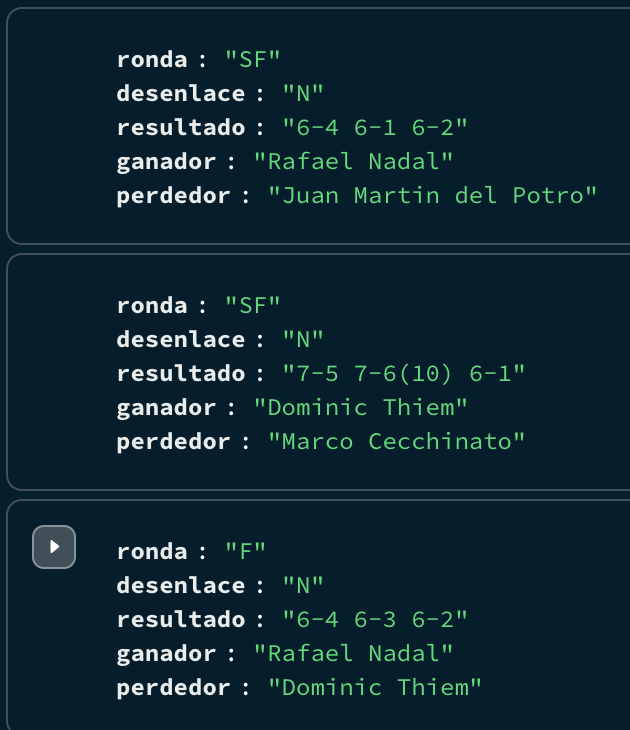
\includegraphics[width=0.4\textwidth]{fotos/mongo/q3.png}
\caption{Bases de datos NoSQL. MongoDB, consulta 3.}
\label{fig:q3_mongo}
\end{figure}


\subsubsection{Muestra la lista de jugadores españoles (ES) que ganaron algún torneo de nivel Gran Slam (G). Para cada jugador muestra los siguientes datos resumen de todos sus partidos: número de partidos jugados, porcentaje de victorias, porcentaje de aces, porcentaje de dobles faltas, porcentaje de servicios ganados, porcentaje de restos ganados, porcentaje de break points salvados (de los sufridos en contra), porcentaje de break points ganados (de los provocados a favor)}

Esta consulta (cuyo resultado mostramos en la figura \ref{fig:q4_mongo} consta de varias etapas en el \texttt{pipeline} de agregación:

\begin{enumerate}
    \item \textbf{\$match:} Filtramos los partidos donde el torneo es de nivel "G" (Grand Slam), la ronda es "F" (final), y el ganador es de España (\texttt{codigo\_iso2} = "ES").
    \item \textbf{\$group:} Agrupamos los documentos por el \texttt{id} del ganador, y para cada grupo obtenemos el nombre completo del jugador (concatenando el \texttt{nombre} y el \texttt{apellido} del ganador) utilizando \texttt{\$first}.
    \item \textbf{\$lookup:} Realizamos una operación de \texttt{join} con la colección \texttt{partidos}, buscando todos los partidos en los que el jugador (basado en su \texttt{id}) haya sido ganador o perdedor. Los resultados los almacenamos en un \textit{array} llamado \texttt{all\_matches}.
    \item \textbf{\$project:} Proyectamos varios campos:
    \begin{itemize}
        \item \texttt{jugador:} El nombre completo del ganador.
        \item \texttt{partidos:} El número de partidos en los que el jugador ha participado, calculado con \texttt{\$size}.
        \item \texttt{pcje\_victorias:} El porcentaje de victorias calculado como la proporción de victorias del jugador sobre el total de partidos jugados, multiplicado por 100.
        \item \texttt{pcje\_aces:} El porcentaje de \textit{aces} ganados, calculado como el total de \textit{aces} en los partidos ganados dividido por el total de puntos servidos.
        \item \texttt{pcje\_dobles\_faltas:} El porcentaje de dobles faltas cometidas, calculado de manera similar a \texttt{pcje\_aces}.
        \item \texttt{pcje\_servicios\_ganados:} El porcentaje de puntos de servicio ganados, basado en los primeros y segundos servicios, calculado por la misma lógica.
        \item \texttt{pcje\_restos\_ganados:} El porcentaje de puntos ganados en los restos de servicio, calculado de manera similar a \texttt{pcje\_servicios\_ganados}.
        \item \texttt{pcje\_breaks\_salvados:} El porcentaje de \textit{breaks} salvados en comparación con los \textit{breaks} enfrentados, calculado con la misma lógica.
        \item \texttt{pcje\_breaks\_ganados:} El porcentaje de \textit{breaks} ganados comparado con los \textit{breaks} enfrentados.
    \end{itemize}
    \item \textbf{\$project (redondeo):} Redondeamos todos los porcentajes calculados en la etapa anterior a un decimal.
\end{enumerate}

\begin{minted}[frame=single, fontsize=\footnotesize]{js}
db.partidos.aggregate([
  {
    $match: {
      "torneo.nivel": "G",
      ronda: "F",
      "ganador.pais.codigo_iso2": "ES",
    },
  },

  {
    $group: {
      _id: "$ganador.id",
      jugador: {
        $first: {
          $concat: ["$ganador.nombre", " ", "$ganador.apellido"],
        },
      },
    },
  },

  {
    $lookup: {
      from: "partidos",
      let: { playerId: "$_id" },
      pipeline: [
        {
          $match: {
            $expr: {
              $or: [
                {
                  $eq: ["$ganador.id", "$$playerId"],
                },
                {
                  $eq: ["$perdedor.id", "$$playerId"],
                },
              ],
            },
          },
        },
      ],
      as: "all_matches",
    },
  },

  {
    $project: {
      _id: 0,
      jugador: 1,
      partidos: { $size: "$all_matches" },
      pcje_victorias: {
        $multiply: [
          {
            $divide: [
              {
                $size: {
                  $filter: {
                    input: "$all_matches",
                    cond: {
                      $eq: ["$$this.ganador.id", "$_id"],
                    },
                  },
                },
              },
              { $size: "$all_matches" },
            ],
          },
          100,
        ],
      },
      pcje_aces: {
        $multiply: [
          {
            $divide: [
              {
                $sum: {
                  $map: {
                    input: "$all_matches",
                    as: "match",
                    in: {
                      $cond: [
                        {
                          $eq: ["$$match.ganador.id", "$_id"],
                        },
                        "$$match.ganador.stats.aces",
                        "$$match.perdedor.stats.aces",
                      ],
                    },
                  },
                },
              },
              {
                $sum: {
                  $map: {
                    input: "$all_matches",
                    as: "match",
                    in: {
                      $cond: [
                        {
                          $eq: ["$$match.ganador.id", "$_id"],
                        },
                        "$$match.ganador.stats.puntos_servidos",
                        "$$match.perdedor.stats.puntos_servidos",
                      ],
                    },
                  },
                },
              },
            ],
          },
          100,
        ],
      },
      pcje_dobles_faltas: {
        $multiply: [
          {
            $divide: [
              {
                $sum: {
                  $map: {
                    input: "$all_matches",
                    as: "match",
                    in: {
                      $cond: [
                        {
                          $eq: ["$$match.ganador.id", "$_id"],
                        },
                        "$$match.ganador.stats.dobles_faltas",
                        "$$match.perdedor.stats.dobles_faltas",
                      ],
                    },
                  },
                },
              },
              {
                $sum: {
                  $map: {
                    input: "$all_matches",
                    as: "match",
                    in: {
                      $cond: [
                        {
                          $eq: ["$$match.ganador.id", "$_id"],
                        },
                        "$$match.ganador.stats.puntos_servidos",
                        "$$match.perdedor.stats.puntos_servidos",
                      ],
                    },
                  },
                },
              },
            ],
          },
          100,
        ],
      },
      pcje_servicios_ganados: {
        $multiply: [
          {
            $divide: [
              {
                $sum: {
                  $map: {
                    input: "$all_matches",
                    as: "match",
                    in: {
                      $cond: [
                        {
                          $eq: ["$$match.ganador.id", "$_id"],
                        },
                        {
                          $add: [
                            "$$match.ganador.stats.primeros_servicios_ganados",
                            "$$match.ganador.stats.segundos_servicios_ganados",
                          ],
                        },
                        {
                          $add: [
                            "$$match.perdedor.stats.primeros_servicios_ganados",
                            "$$match.perdedor.stats.segundos_servicios_ganados",
                          ],
                        },
                      ],
                    },
                  },
                },
              },
              {
                $sum: {
                  $map: {
                    input: "$all_matches",
                    as: "match",
                    in: {
                      $cond: [
                        {
                          $eq: ["$$match.ganador.id", "$_id"],
                        },
                        "$$match.ganador.stats.puntos_servidos",
                        "$$match.perdedor.stats.puntos_servidos",
                      ],
                    },
                  },
                },
              },
            ],
          },
          100,
        ],
      },
      pcje_restos_ganados: {
        $multiply: [
          {
            $divide: [
              {
                $sum: {
                  $map: {
                    input: "$all_matches",
                    as: "match",
                    in: {
                      $cond: [
                        {
                          $eq: ["$$match.ganador.id", "$_id"],
                        },
                        {
                          $subtract: [
                            "$$match.perdedor.stats.puntos_servidos",
                            {
                              $add: [
                                "$$match.perdedor.stats.primeros_servicios_ganados",
                                "$$match.perdedor.stats.segundos_servicios_ganados",
                              ],
                            },
                          ],
                        },
                        {
                          $subtract: [
                            "$$match.ganador.stats.puntos_servidos",
                            {
                              $add: [
                                "$$match.ganador.stats.primeros_servicios_ganados",
                                "$$match.ganador.stats.segundos_servicios_ganados",
                              ],
                            },
                          ],
                        },
                      ],
                    },
                  },
                },
              },
              {
                $sum: {
                  $map: {
                    input: "$all_matches",
                    as: "match",
                    in: {
                      $cond: [
                        {
                          $eq: ["$$match.ganador.id", "$_id"],
                        },
                        "$$match.perdedor.stats.puntos_servidos",
                        "$$match.ganador.stats.puntos_servidos",
                      ],
                    },
                  },
                },
              },
            ],
          },
          100,
        ],
      },
      pcje_breaks_salvados: {
        $multiply: [
          {
            $divide: [
              {
                $sum: {
                  $map: {
                    input: "$all_matches",
                    as: "match",
                    in: {
                      $cond: [
                        {
                          $eq: ["$$match.ganador.id", "$_id"],
                        },
                        "$$match.ganador.stats.breaks_salvados",
                        "$$match.perdedor.stats.breaks_salvados",
                      ],
                    },
                  },
                },
              },
              {
                $sum: {
                  $map: {
                    input: "$all_matches",
                    as: "match",
                    in: {
                      $cond: [
                        {
                          $eq: ["$$match.ganador.id", "$_id"],
                        },
                        "$$match.ganador.stats.breaks_afrontados",
                        "$$match.perdedor.stats.breaks_afrontados",
                      ],
                    },
                  },
                },
              },
            ],
          },
          100,
        ],
      },
      pcje_breaks_ganados: {
        $multiply: [
          {
            $divide: [
              {
                $sum: {
                  $map: {
                    input: "$all_matches",
                    as: "match",
                    in: {
                      $cond: [
                        {
                          $eq: ["$$match.ganador.id", "$_id"],
                        },
                        {
                          $subtract: [
                            "$$match.perdedor.stats.breaks_afrontados",
                            "$$match.perdedor.stats.breaks_salvados",
                          ],
                        },
                        {
                          $subtract: [
                            "$$match.ganador.stats.breaks_afrontados",
                            "$$match.ganador.stats.breaks_salvados",
                          ],
                        },
                      ],
                    },
                  },
                },
              },
              {
                $sum: {
                  $map: {
                    input: "$all_matches",
                    as: "match",
                    in: {
                      $cond: [
                        {
                          $eq: ["$$match.ganador.id", "$_id"],
                        },
                        "$$match.perdedor.stats.breaks_afrontados",
                        "$$match.ganador.stats.breaks_afrontados",
                      ],
                    },
                  },
                },
              },
            ],
          },
          100,
        ],
      },
    },
  },

  // Round all percentages to 1 decimal place
  {
    $project: {
      jugador: 1,
      partidos: 1,
      pcje_victorias: {
        $round: ["$pcje_victorias", 1],
      },
      pcje_aces: { $round: ["$pcje_aces", 1] },
      pcje_dobles_faltas: {
        $round: ["$pcje_dobles_faltas", 1],
      },
      pcje_servicios_ganados: {
        $round: ["$pcje_servicios_ganados", 1],
      },
      pcje_restos_ganados: {
        $round: ["$pcje_restos_ganados", 1],
      },
      pcje_breaks_salvados: {
        $round: ["$pcje_breaks_salvados", 1],
      },
      pcje_breaks_ganados: {
        $round: ["$pcje_breaks_ganados", 1],
      },
    },
  },
]);
\end{minted}

\begin{figure}[H]
\centering
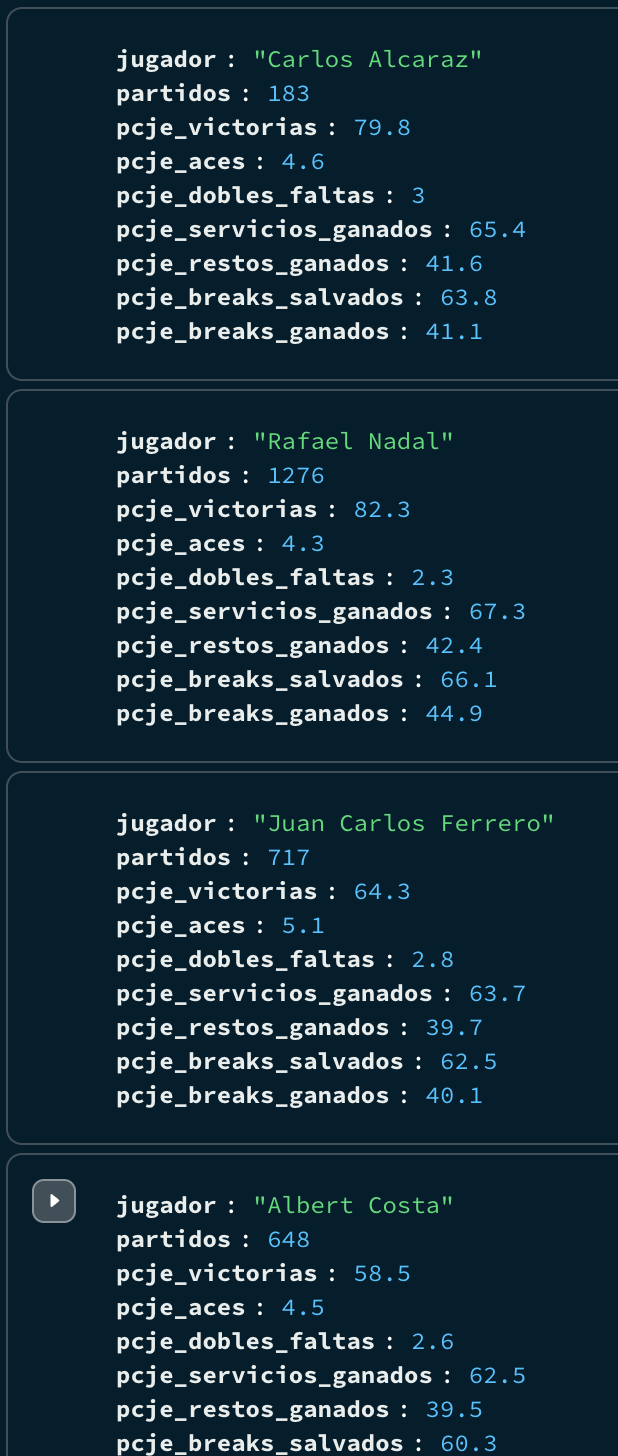
\includegraphics[width=0.3\textwidth]{fotos/mongo/q4.png}
\caption{Bases de datos NoSql. MongoDB, consulta 4. Resultado parcial debido al tamaño del mismo.}
\label{fig:q4_mongo}
\end{figure}




\subsubsection{Lista los jugadores que fueron derrotados (en algún partido del 2018) por el rival de Rafael Nadal de la primera ronda (R128) de Roland Garros de 2018}

Esta consulta (cuyo resultado mostramos en la figura \ref{fig:q5_mongo}) consta de varias etapas en el \texttt{pipeline} de agregación:

\begin{enumerate}
    \item \textbf{\$match:} Filtramos los partidos del torneo \texttt{"Roland Garros"} en el año 2018, específicamente de la ronda \texttt{R128}, y donde al menos uno de los jugadores es \texttt{Rafael Nadal}, ya sea como ganador o perdedor.
    \item \textbf{\$project:} Agregamos un campo \texttt{rival\_id} que determina el \texttt{id} del rival del jugador \texttt{Rafael Nadal}. Si \texttt{Rafael Nadal} es el ganador del partido, se asigna el \texttt{id} del perdedor; de lo contrario, se asigna el \texttt{id} del ganador.
    
    \item \textbf{\$lookup:} Realizamos una operación de \texttt{join} con la colección \texttt{partidos}, buscando los partidos donde el \texttt{id} del rival aparece como ganador. El resultado de esta operación se almacena en el campo \texttt{partidos\_rival}.
    
    \item \textbf{\$unwind:} Descomponemos el \textit{array} \texttt{partidos\_rival} para obtener un único documento por cada partido encontrado. Esto convierte los elementos del \textit{array} en documentos separados dentro del flujo.
    \item \textbf{\$match:} Filtramos los documentos para asegurarse de que los partidos de la colección \texttt{partidos\_rival} sean del año 2018, usando el operador \texttt{\$year} en la fecha del torneo.
    \item \textbf{\$project:} Proyectamos el nombre y apellido del \texttt{perdedor} de cada partido del rival, concatenando ambos en un solo campo \texttt{jugador}. También proyectamos el código de país (\texttt{codigo\_iso2}) del \texttt{perdedor} del partido del rival.
\end{enumerate}

\begin{minted}[frame=single, fontsize=\footnotesize]{js}
db.partidos.aggregate([
  {
    $match: {
      "torneo.nombre": "Roland Garros",
      $expr: {
        $eq: [{ $year: { $toDate: "$torneo.fecha" } }, 2018],
      },
      ronda: "R128",
      $or: [
        {
          "ganador.nombre": "Rafael",
          "ganador.apellido": "Nadal",
        },
        {
          "perdedor.nombre": "Rafael",
          "perdedor.apellido": "Nadal",
        },
      ],
    },
  },

  {
    $project: {
      rival_id: {
        $cond: [
          {
            $and: [
              {
                $eq: ["$ganador.nombre", "Rafael"],
              },
              {
                $eq: ["$ganador.apellido", "Nadal"],
              },
            ],
          },
          "$perdedor.id",
          "$ganador.id",
        ],
      },
    },
  },

  {
    $lookup: {
      from: "partidos",
      localField: "rival_id",
      foreignField: "ganador.id",
      as: "partidos_rival",
    },
  },
  {
    $unwind: "$partidos_rival",
  },
  {
    $match: {
      $expr: {
        $eq: [
          {
            $year: {
              $toDate: "$partidos_rival.torneo.fecha",
            },
          },
          2018,
        ],
      },
    },
  },
  {
    $project: {
      _id: 0,
      jugador: {
        $concat: [
          "$partidos_rival.perdedor.nombre",
          " ",
          "$partidos_rival.perdedor.apellido",
        ],
      },
      pais: "$partidos_rival.perdedor.pais.codigo_iso2",
    },
  },
]);
\end{minted}

\begin{figure}[H]
\centering
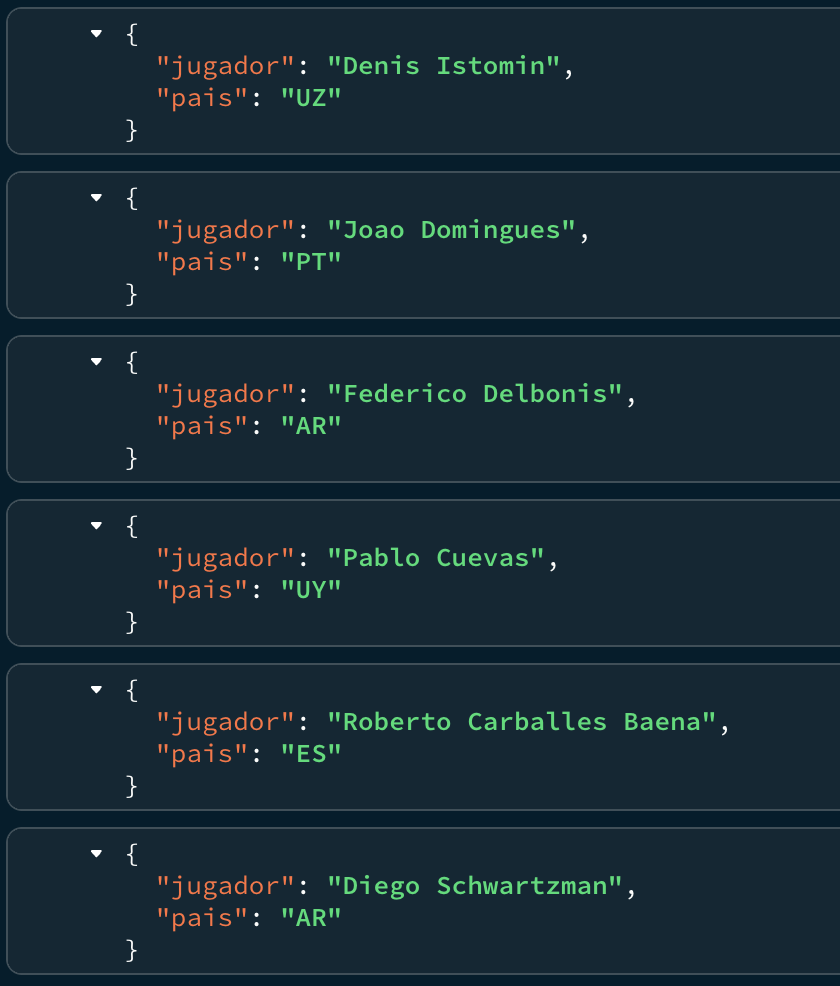
\includegraphics[width=0.38\textwidth]{fotos/mongo/q5.png}
\caption{Bases de datos NoSQL. MongoDB, consulta 5.}
\label{fig:q5_mongo}
\end{figure}



\subsection{Preferencias y compromiso de lectura}

Procedemos ahora a comprobar si el \textit{cluster} sigue funcionando al retirar nodos. Para probar esto, creamos una consulta de prueba que fuerce a MongoDB a emplear datos de todos los \textit{shards}. La consulta que planteamos agrega el total de partidos con desenlace normal:

\begin{minted}[frame=single, fontsize=\footnotesize]{js}
db.partidos.aggregate([  
    {$match: { desenlace: "N" } },
    {$count: "partidos_con_desenlace_normal"},
]);
\end{minted}

Procedemos a parar todos los procesos de MongoDB en un nodo como ya hemos visto anteriormente, y comprobamos que la consulta sigue ejecutándose correctamente. Al dejar un solo nodo activo, la consulta ya no puede ejecutarse y nos devuelve un error (ver figura \ref{fig:error_mongoD}).

\begin{figure}[H]
\centering
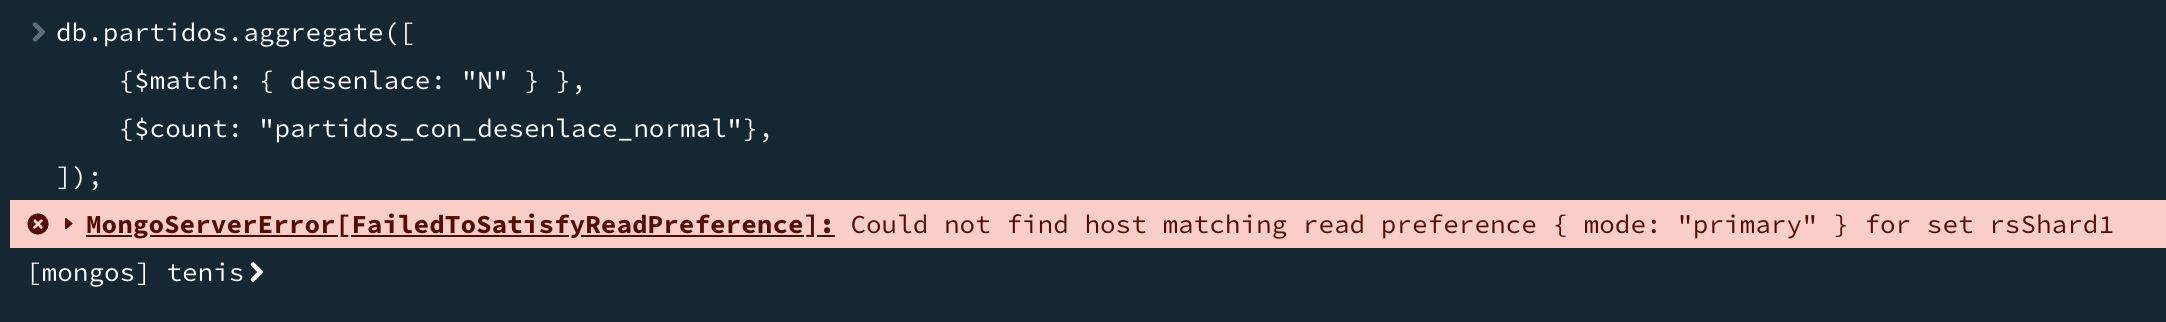
\includegraphics[width=0.9\textwidth]{fotos/mongo/1_node_Error.png}
\caption{Error en MongoDB al retirar nodos.}
\label{fig:error_mongoD}
\end{figure}

Comprobamos cuál es la preferencia de lectura, que por defecto está configurada para leer desde el primario, y el compromiso de lectura, por defecto, lectura local sin garantía de leer los datos más recientes (figura \ref{fig:comprobarpermisos}.

\begin{figure}[H]
     \centering
     \begin{subfigure}[b]{0.45\textwidth}
        \centering
        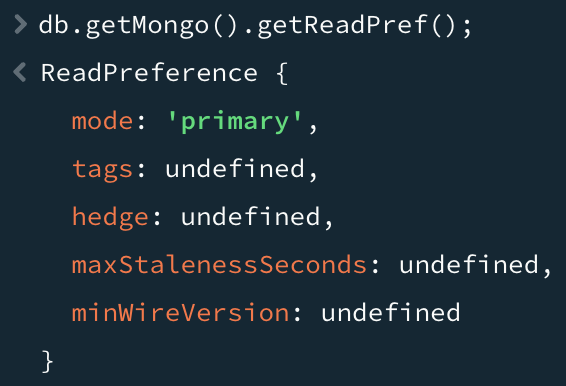
\includegraphics[width=\textwidth]{fotos/mongo/read_pref_default.png}
        \caption{Preferencias de lectura en nuestro \textit{cluster}.}
     \end{subfigure}
     \hfill
     \begin{subfigure}[b]{0.45\textwidth}
        \centering
        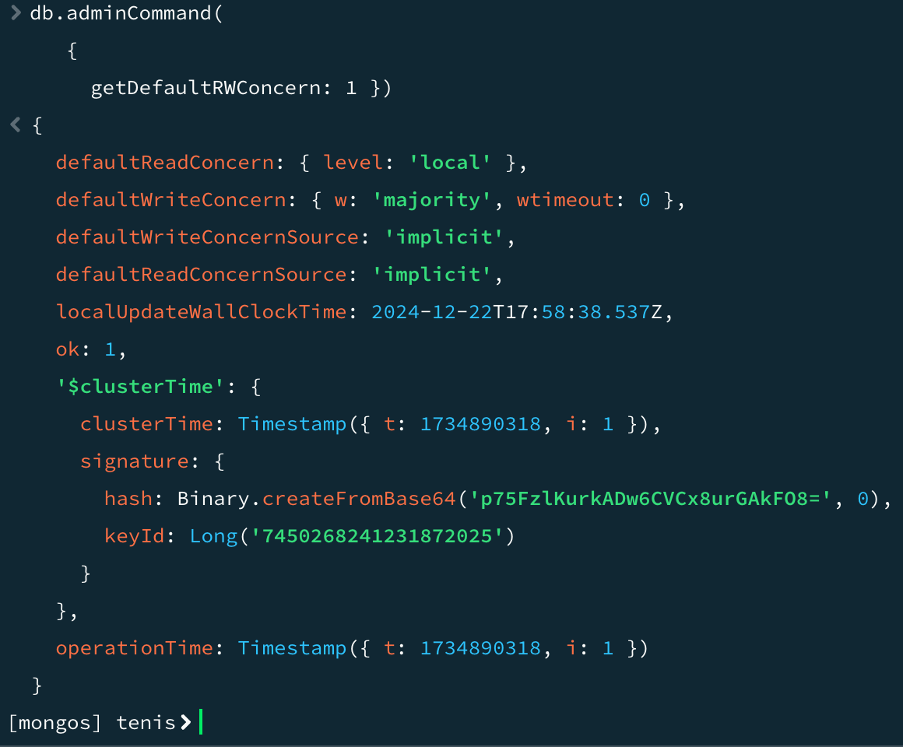
\includegraphics[width=\textwidth]{fotos/mongo/Picture 1.png}
        \caption{Compromiso de lectura en nuestro \textit{cluster}.}
     \end{subfigure}
\caption{Verificación de nodos del \textit{cluster}.}
\label{fig:comprobarpermisos}
\end{figure}

Podemos concluir que uno de los nodos eliminados era el primario, y que el nodo que queda vivo es un secundario que no ha sido capaz de promocionarse a primario, ya que no quedan nodos vivos con los cuales comunicarse para establecer una votación. \\

Si cambiamos las preferencias de lectura a cualquiera que no obligue a leer del primario, las consultas volverán a funcionar (figura \ref{fig:mongo_prueba}).

\begin{figure}[H]
\centering
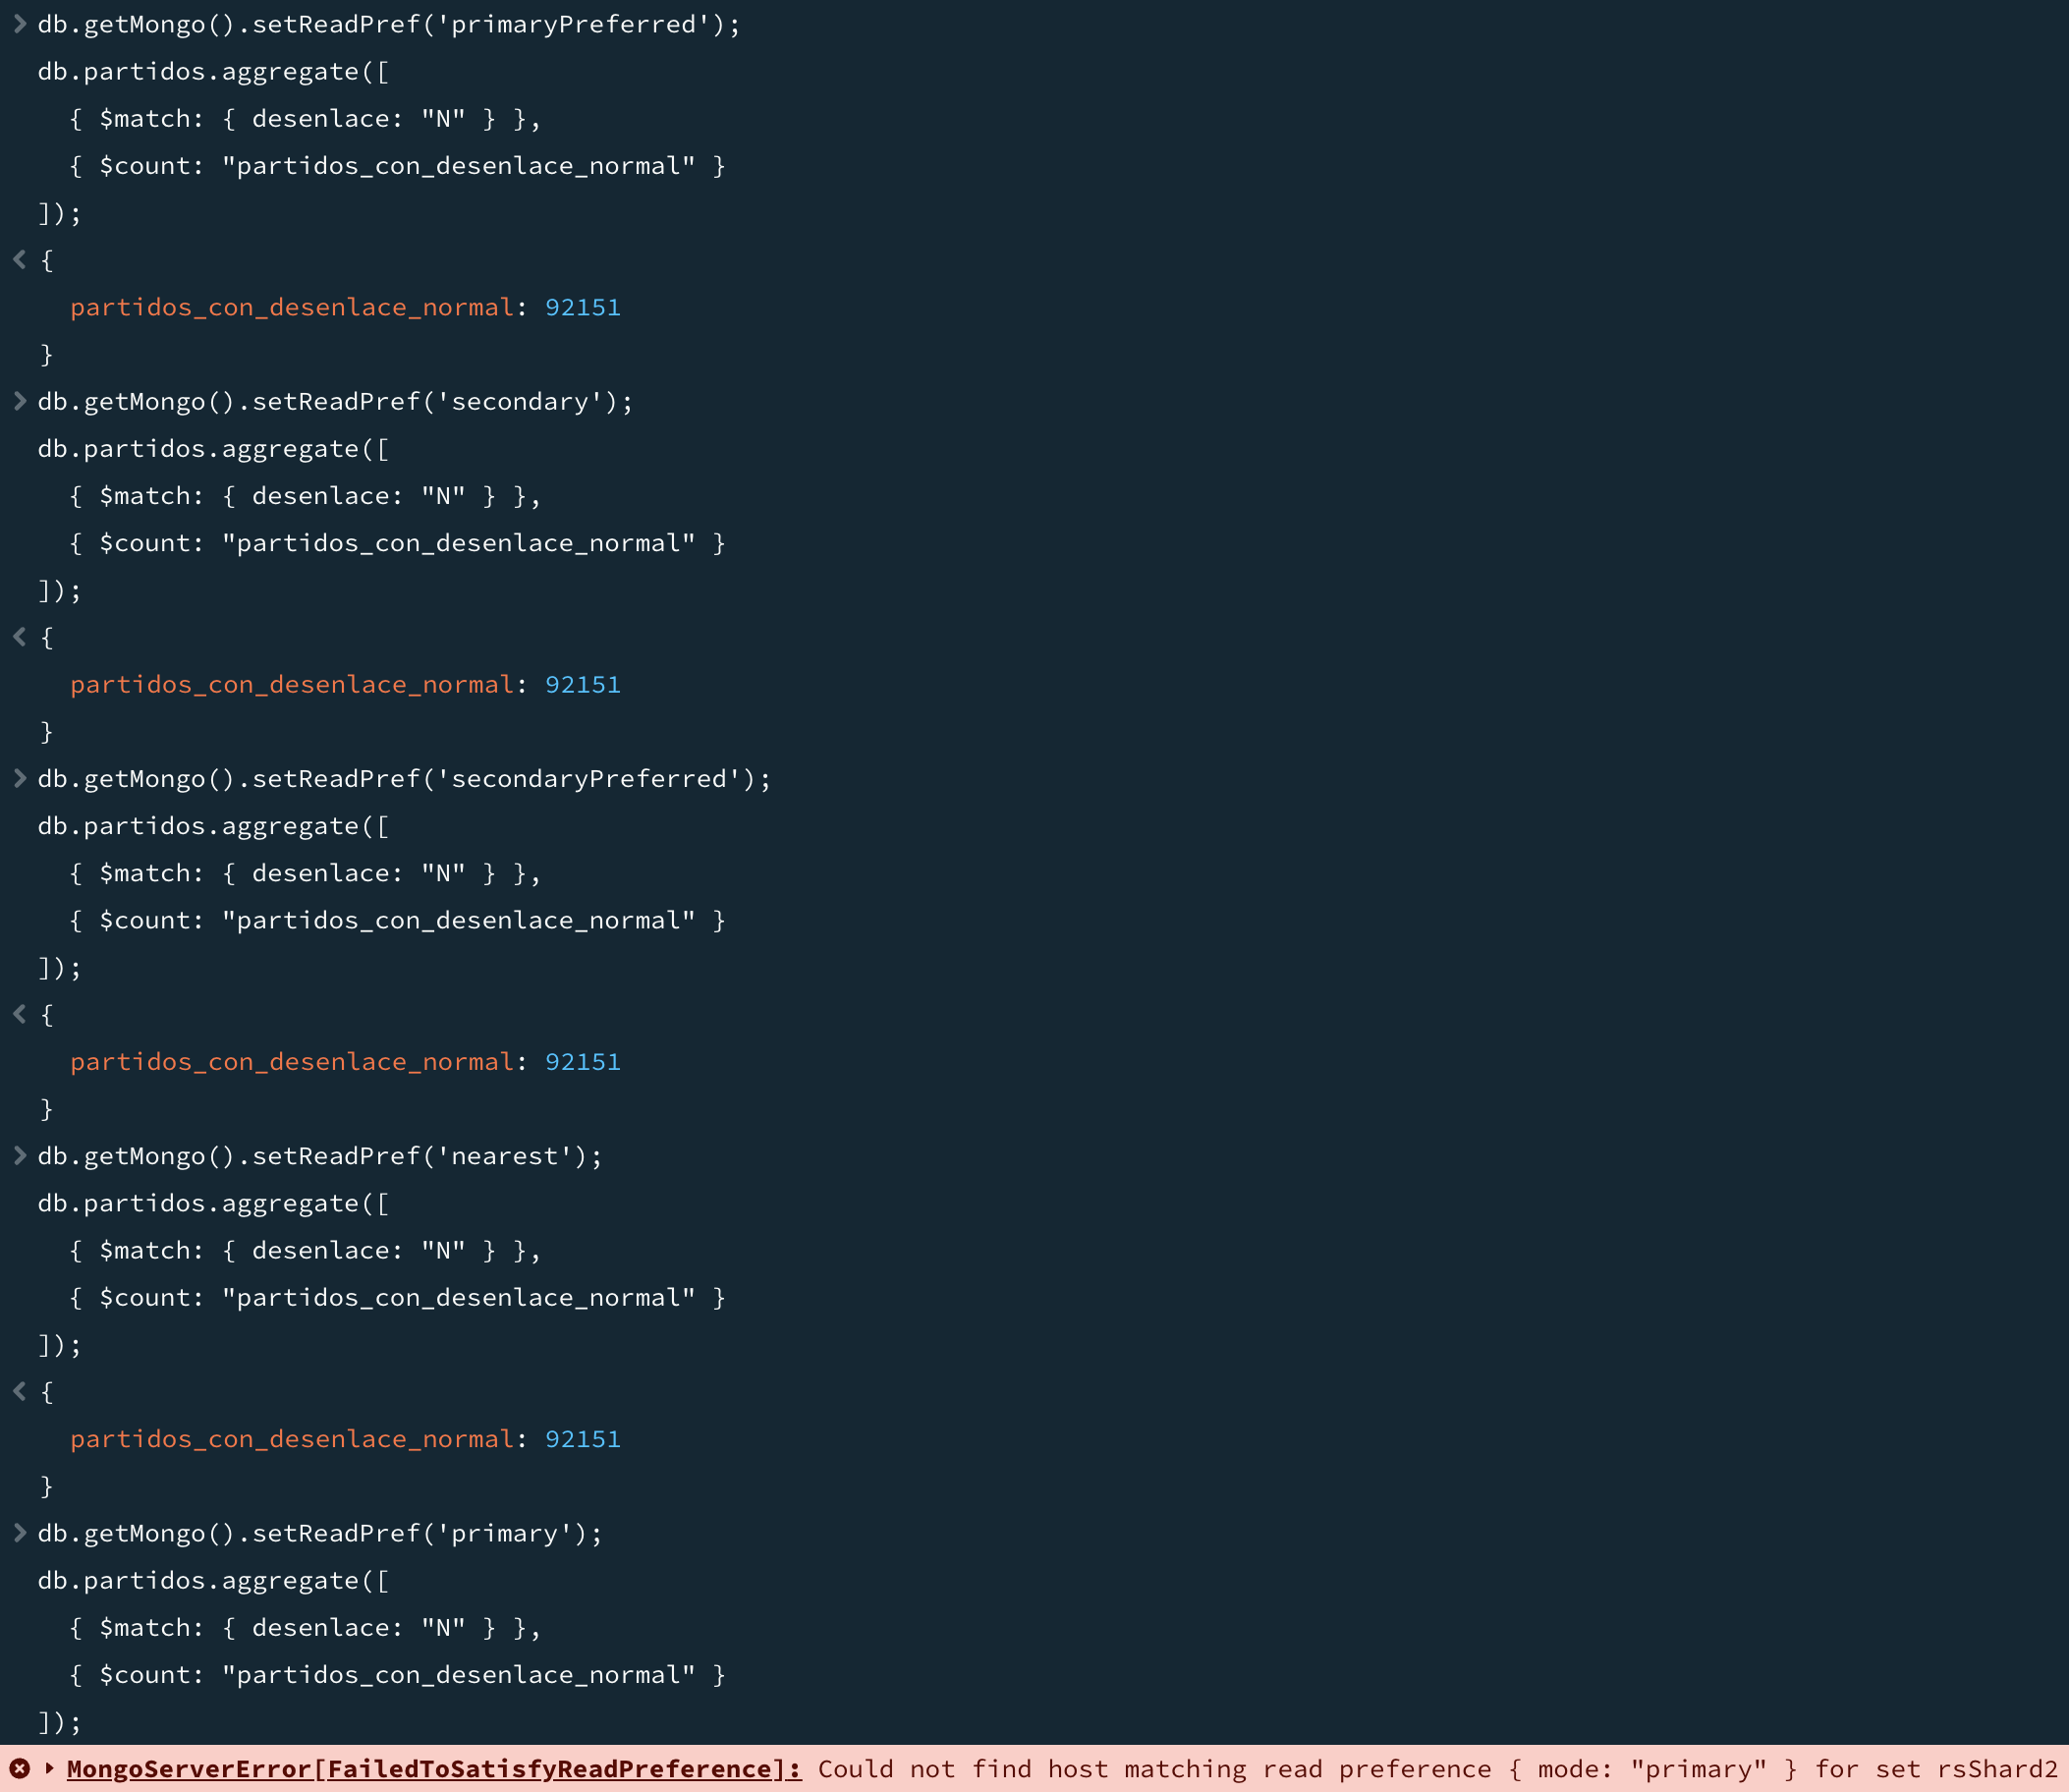
\includegraphics[width=0.7\textwidth]{fotos/mongo/readPRefsResults.png}
\caption{Resultados de consulta de prueba.}
\label{fig:mongo_prueba}
\end{figure}

Fijando la preferencia de lectura en \textbf{primaryPreferred}, procedemos ahora a ver cómo afecta el compromiso de lectura a la posibilidad de ejecutar la consulta.

\begin{figure}[H]
\centering
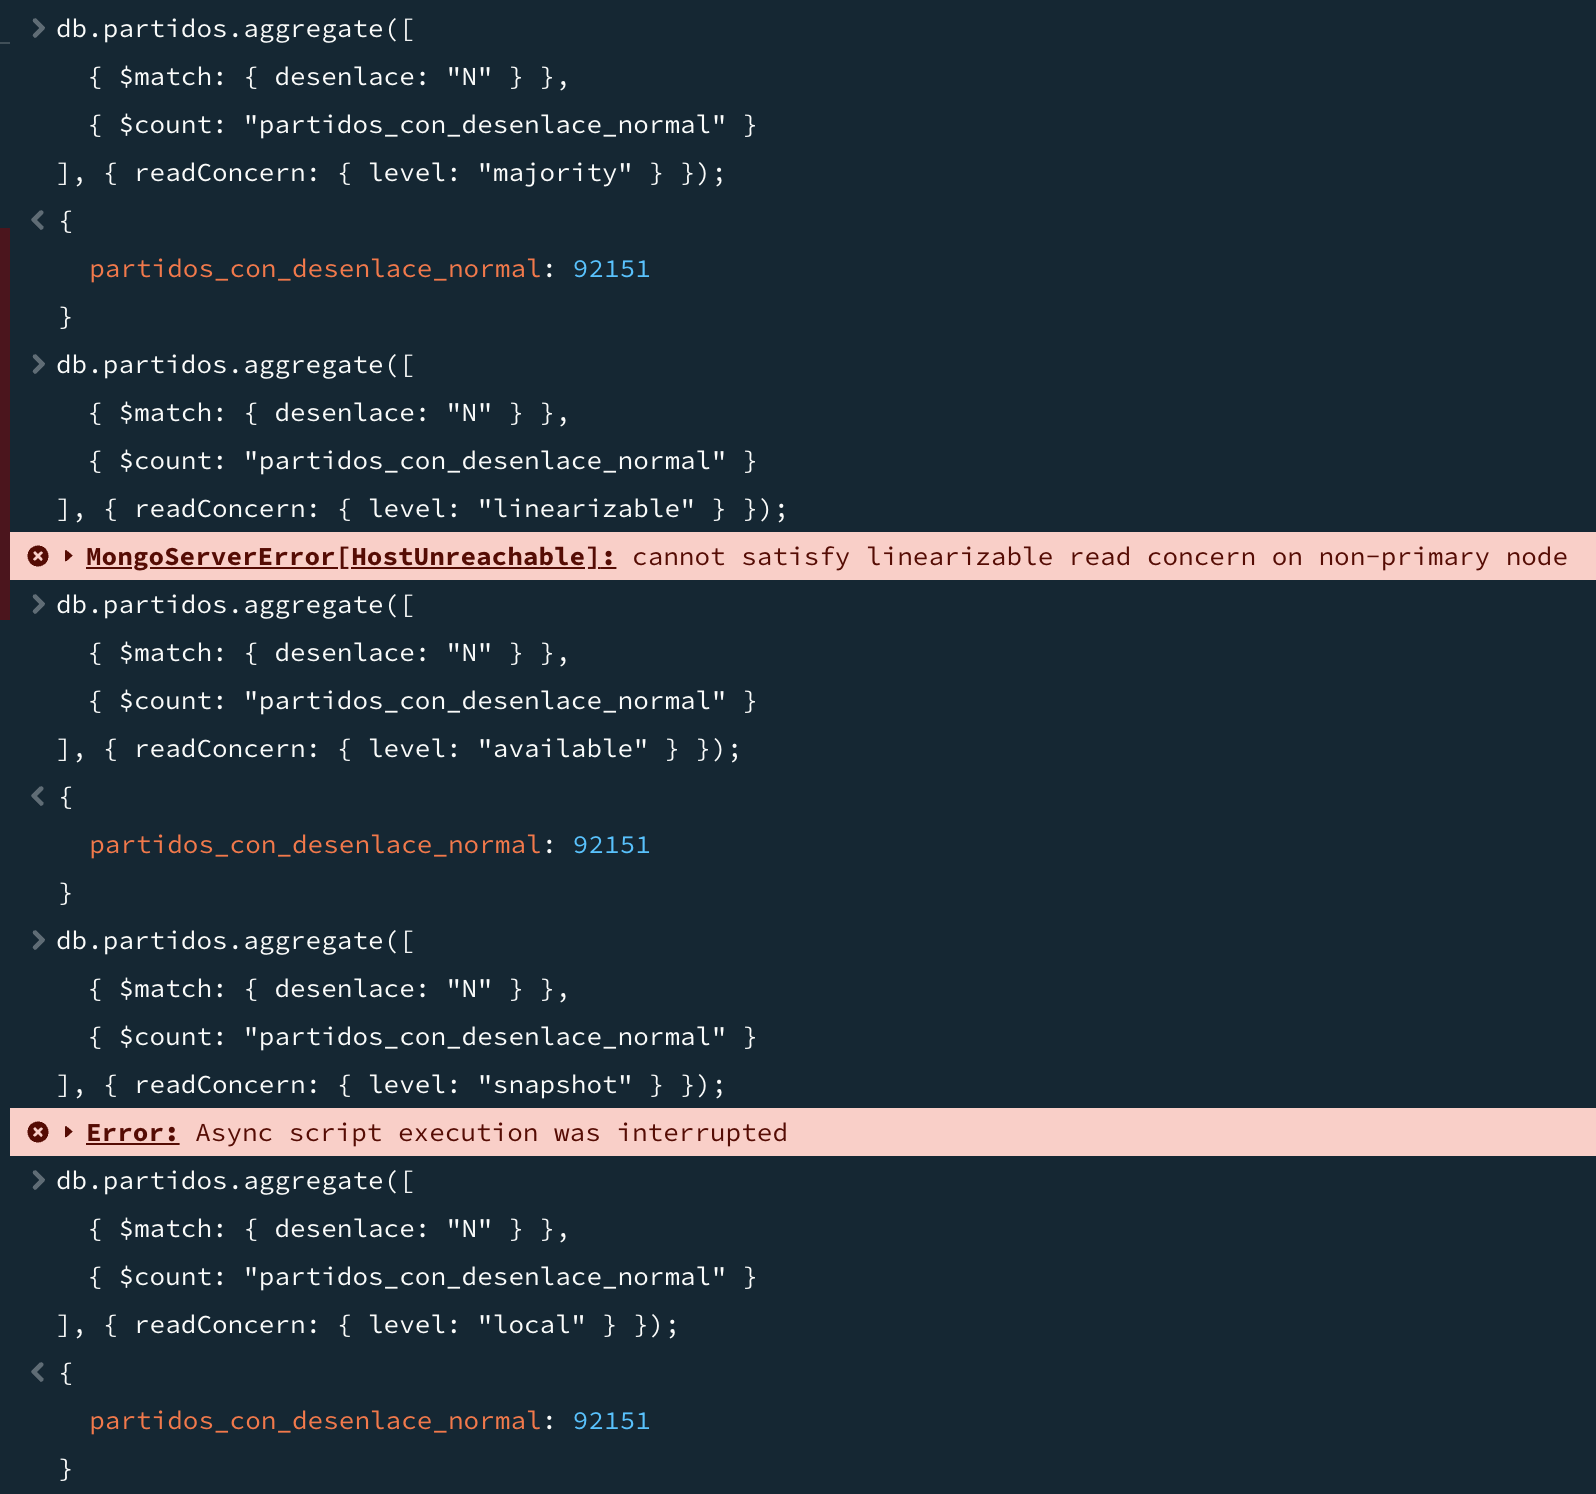
\includegraphics[width=0.55\textwidth]{fotos/mongo/read_concerns.png}
\caption{Efecto del compromiso de lectura al ejecutar la consulta.}
\label{fig:mongo_concerns}
\end{figure}

El compromiso de lectura \texttt{linearizable}, que nos garantiza leer los datos más recientes, falla, ya que este solo puede especificarse para operaciones de lectura desde el primario. También falla el compromiso de lectura \texttt{snapshot}, que requiere confirmar que los datos están en un estado consistente, cosa imposible con un solo nodo secundario, dado que no existe el \textit{quorum} necesario para garantizar esta consistencia.
